\chapter{Re:VIEW Starterの独自機能}
\label{chap:chap01-starter}
\begin{starterabstract}
素のRe:VIEWと比べて、Re:VIEW Starter(以下「Starter」とする)はいろんな機能強化やバグフィックスをしています。
この章では、それらについて解説します\footnote{本章では、Re:VIEWや\LaTeX{}についての説明はしません。Re:VIEWの書き方についてはマニュアル(\url{https://github.com/kmuto/review/blob/master/doc/format.ja.md})やチートシート(\url{https://qiita.com/froakie0021/items/b0f4ba5f242bbd571d4e})を参照してください。}。

また本章ではRe:VIEWの機能や\LaTeX{}の用語が説明なく使われます。
これらが分からなければ読み飛ばして、分かる箇所だけ読んでください。
\end{starterabstract}

\section{原稿本文を書くための機能}
\label{sec:1-1}
\label{sec-ext}

\subsection*{強調}
\addcontentsline{toc}{subsection}{強調}
\label{sec:1-1-1}

\begin{starteritemize}
\item 「\texttt{@\textless{}b\textgreater{}\{...\}}」は、明朝体のまま太字になります(Re:VIEWのデフォルト)。
\item 「\texttt{@\textless{}em\textgreater{}\{...\}}」は、ゴシック体になります(Starter拡張)。
\item 「\texttt{@\textless{}strong\textgreater{}\{...\}}」は、太字のゴシック体になります(Starter拡張)。
\item 「\texttt{@\textless{}B\textgreater{}\{...\}}」は、「\texttt{@\textless{}strong\textgreater{}\{...\}}」のショートカットです(Starter拡張)。
\end{starteritemize}

\startercodeblockcaption{サンプル}
\begin{starterprogram}\seqsplit{いろはfghij  @\textless{}b\textgreater{}\{いろはfghij\}  @\textless{}em\textgreater{}\{いろはfghij\}  @\textless{}strong\textgreater{}\{いろはfghij\}
@\textless{}B\textgreater{}\{いろはfghij\}}\end{starterprogram}
\noindent
\reviewem{表示結果:}

\starterresult

いろはfghij  \textbf{いろはfghij}  \reviewem{いろはfghij}  \reviewstrong{いろはfghij}
\reviewstrong{いろはfghij}

\endstarterresult

なおソースコードの一部を太字にしたいときは、「\texttt{@\textless{}strong\textgreater{}\{...\}}」ではなく「\texttt{@\textless{}b\textgreater{}\{...\}}」を使ってください。
なぜなら「\texttt{@\textless{}strong\textgreater{}\{...\}}」だとゴシック体になってしまうのに対し、「\texttt{@\textless{}b\textgreater{}\{...\}}」だとタイプライタ体のまま太字になるからです。

\startercodeblockcaption{サンプル}
\begin{starterprogram}\seqsplit{//emlist\{
タイプライタ体(通常): 0123456789 ijkl IJKL !"\textdollar{}\%\&()*,{-}./:;?@[\reviewbackslash{}]`\textbar{}\textasciitilde{}
タイプライタ体(太字): @\textless{}b\textgreater{}\{0123456789 ijkl IJKL !"\textdollar{}\%\&()*,{-}./:;?@[\reviewbackslash{}\reviewbackslash{}]`\textbar{}\textasciitilde{}\}
ゴシック体  (太字): @\textless{}strong\textgreater{}\{0123456789 ijkl IJKL !"\textdollar{}\%\&()*,{-}./:;?@[\reviewbackslash{}\reviewbackslash{}]`\textbar{}\textasciitilde{}\}
//\}}\end{starterprogram}
\noindent
\reviewem{表示結果:}

\starterresult
\begin{starterprogram}\seqsplit{タイプライタ体(通常): 0123456789 ijkl IJKL !"\textdollar{}\%\&()*,{-}./:;?@[\reviewbackslash{}]`\textbar{}\textasciitilde{}
タイプライタ体(太字): \bfseries{}0123456789 ijkl IJKL !"\textdollar{}\%\&()*,{-}./:;?@[\reviewbackslash{}]`\textbar{}\textasciitilde{}\mdseries{}
ゴシック体  (太字): \reviewstrong{0123456789 ijkl IJKL !"\textdollar{}\%\&()*,{-}./:;?@[\reviewbackslash{}]`\textbar{}\textasciitilde{}}}\end{starterprogram}
\endstarterresult

\subsection*{目立たせないための「\texttt{@\textless{}weak\textgreater{}\{\}}」}
\addcontentsline{toc}{subsection}{目立たせないための「\texttt{@\textless{}weak\textgreater{}\{\}}」}
\label{sec:1-1-2}

強調とは逆に、テキストを目立たせないための「\texttt{@\textless{}weak\textgreater{}\{\}}」という命令も用意しました。
いわゆる「おまじない」のコードを目立たなくさせるときに使うといいでしょう。

次のはPHPのおまじないを目立たなくした例です。

\startercodeblockcaption{サンプル}
\begin{starterprogram}\seqsplit{//list[][PHPサンプルコード]\{
\bfseries{}@\mdseries{}\bfseries{}\textless{}weak\textgreater{}\{\mdseries{}\textless{}?php\bfseries{}\}\mdseries{}
function fib(\textdollar{}n) \{
    return \textdollar{}n \textless{}= 1 ? \textdollar{}n : fib(\textdollar{}n{-}1) + fib(\textdollar{}n{-}2);
\}
\bfseries{}@\mdseries{}\bfseries{}\textless{}weak\textgreater{}\{\mdseries{}?\textgreater{}\bfseries{}\}\mdseries{}
//\}}\end{starterprogram}
\noindent
\reviewem{表示結果:}

\starterresult
\startercodeblockcaption{PHPサンプルコード}
\label{}
\begin{starterprogram}\seqsplit{{\starterweak{\seqsplit{\textless{}?php}}}
function fib(\textdollar{}n) \{
    return \textdollar{}n \textless{}= 1 ? \textdollar{}n : fib(\textdollar{}n{-}1) + fib(\textdollar{}n{-}2);
\}
{\starterweak{\seqsplit{?\textgreater{}}}}}\end{starterprogram}
\endstarterresult

次のはJavaのおまじないを目立たなくした例です。

\startercodeblockcaption{サンプル}
\begin{starterprogram}\seqsplit{//list[][Javaサンプルコード]\{
\bfseries{}@\mdseries{}\bfseries{}\textless{}weak\textgreater{}\textdollar{}\mdseries{}public class Example \{\bfseries{}\textdollar{}\mdseries{}
    \bfseries{}@\mdseries{}\bfseries{}\textless{}weak\textgreater{}\textdollar{}\mdseries{}public static void main(String[] args) \{\bfseries{}\textdollar{}\mdseries{}
        System.out.println("Hello!");
    \bfseries{}@\mdseries{}\bfseries{}\textless{}weak\textgreater{}\textdollar{}\mdseries{}\}\bfseries{}\textdollar{}\mdseries{}
\bfseries{}@\mdseries{}\bfseries{}\textless{}weak\textgreater{}\textdollar{}\mdseries{}\}\bfseries{}\textdollar{}\mdseries{}
//\}}\end{starterprogram}
\noindent
\reviewem{表示結果:}

\starterresult
\startercodeblockcaption{Javaサンプルコード}
\label{}
\begin{starterprogram}\seqsplit{{\starterweak{\seqsplit{public class Example \{}}}
    {\starterweak{\seqsplit{public static void main(String[] args) \{}}}
        System.out.println("Hello!");
    {\starterweak{\seqsplit{\}}}}
{\starterweak{\seqsplit{\}}}}}\end{starterprogram}
\endstarterresult

\subsection*{番号つきリストの機能強化}
\addcontentsline{toc}{subsection}{番号つきリストの機能強化}
\label{sec:1-1-3}
\label{subsec-olist}

Re:VIEWでは番号つきリストを次のように書きます。

\startercodeblockcaption{サンプル}
\begin{starterprogram}\seqsplit{ 1. XXX
 2. YYY
 3. ZZZ}\end{starterprogram}
\noindent
\reviewem{表示結果:}

\starterresult

\begin{starterenumerate}
\item XXX
\item YYY
\item ZZZ
\end{starterenumerate}

\endstarterresult

この書き方には次の欠点があります。

\begin{starteritemize}
\item 数字の番号はつきますが、「A.」や「a.」などは使えません。
\item また番号つきリストを入れ子にできません。
\end{starteritemize}

そこでStarterでは別の書き方を用意しました。

\startercodeblockcaption{サンプル}
\begin{starterprogram}\seqsplit{数字による番号つきリスト

 {-} 1. XXX
 {-} 2. YYY
 {-} 3. ZZZ

大文字による番号つきリスト

 {-} A. XXX
 {-} B. YYY
 {-} C. ZZZ

小文字による番号つきリスト

 {-} a. XXX
 {-} b. YYY
 {-} c. ZZZ}\end{starterprogram}
\noindent
\reviewem{表示結果:}

\starterresult

数字による番号つきリスト

\begin{starterenumerate}
\item[1.] XXX
\item[2.] YYY
\item[3.] ZZZ
\end{starterenumerate}

大文字による番号つきリスト

\begin{starterenumerate}
\item[A.] XXX
\item[B.] YYY
\item[C.] ZZZ
\end{starterenumerate}

小文字による番号つきリスト

\begin{starterenumerate}
\item[a.] XXX
\item[b.] YYY
\item[c.] ZZZ
\end{starterenumerate}

\endstarterresult

「1.」や「A.」や「a.」のあとに必ず半角空白が必要です。
実は半角空白があれば、その前に書いた文字列がそのまま出力されます。
なので次のような書き方もできます。
箇条書きのように見えますが、「・」がついてないことに注意してください。

\startercodeblockcaption{サンプル}
\begin{starterprogram}\seqsplit{ {-} (A) 項目A
 {-} (B) 項目B
 {-} (C) 項目C

 {-} 甲: 山田太郎
 {-} 乙: 佐藤花子}\end{starterprogram}
\noindent
\reviewem{表示結果:}

\starterresult

\begin{starterenumerate}
\item[(A)] 項目A
\item[(B)] 項目B
\item[(C)] 項目C
\end{starterenumerate}

\begin{starterenumerate}
\item[甲:] 山田太郎
\item[乙:] 佐藤花子
\end{starterenumerate}

\endstarterresult

また入れ子にできます。

\startercodeblockcaption{サンプル}
\begin{starterprogram}\seqsplit{ {-} (A) 作業A
 {-}{-} (A{-}1) 作業A{-}1
 {-}{-} (A{-}2) 作業A{-}2}\end{starterprogram}
\noindent
\reviewem{表示結果:}

\starterresult

\begin{starterenumerate}
\item[(A)] 作業A

\begin{starterenumerate}
\item[(A{-}1)] 作業A{-}1
\item[(A{-}2)] 作業A{-}2
\end{starterenumerate}

\end{starterenumerate}

\endstarterresult

箇条書きとの混在もできます。

\startercodeblockcaption{サンプル}
\begin{starterprogram}\seqsplit{番号つきリストの中に箇条書き

 {-} A. XXX
 ** xxx
 ** xxx

箇条書きの中に番号つきリスト

 * XXXX
 {-}{-} a. xxx
 {-}{-} b. xxx}\end{starterprogram}
\noindent
\reviewem{表示結果:}

\starterresult

番号つきリストの中に箇条書き

\begin{starterenumerate}
\item[A.] XXX

\begin{starteritemize}
\item xxx
\item xxx
\end{starteritemize}

\end{starterenumerate}

箇条書きの中に番号つきリスト

\begin{starteritemize}
\item XXXX

\begin{starterenumerate}
\item[a.] xxx
\item[b.] xxx
\end{starterenumerate}

\end{starteritemize}

\endstarterresult

なお数字や大文字や小文字の順番を補正するようなことはしません。
たとえば「1.」を連続して書けばそれがそのまま出力されます。

\startercodeblockcaption{サンプル}
\begin{starterprogram}\seqsplit{ {-} 1. XXX
 {-} 1. YYY
 {-} 1. ZZZ}\end{starterprogram}
\noindent
\reviewem{表示結果:}

\starterresult

\begin{starterenumerate}
\item[1.] XXX
\item[1.] YYY
\item[1.] ZZZ
\end{starterenumerate}

\endstarterresult

\subsection*{ノート}
\addcontentsline{toc}{subsection}{ノート}
\label{sec:1-1-4}
\label{subsec-ext-note}

「\texttt{//note[}...\texttt{]\{} ... \texttt{//\}}」で、付加情報や注意書きのブロックが書けます。
Re:VIEW標準と比べると、デザインを大きく変更していることと、段落の先頭は1文字分インデントされる点が違います。

\startercodeblockcaption{サンプル}
\begin{starterprogram}\seqsplit{//note[■注意:印刷所の締切り日を確かめること]\{
印刷所の締切りは、技術書典のようなイベントの本番当日よりずっと前です。
通常は約1週間前、また割引きを受けようと思ったら約2週間前が締切りです。
実際の締切り日は印刷所ごとに違うので、必ず確認しておきましょう。

また他の人に原稿のレビューを頼む場合は、さらに1〜2週間必要です。
これも忘れやすいので注意しましょう。
//\}}\end{starterprogram}
\noindent
\reviewem{表示結果:}

\starterresult
\begin{starternote}{■注意:印刷所の締切り日を確かめること}
\begin{starternoteinner}

印刷所の締切りは、技術書典のようなイベントの本番当日よりずっと前です。
通常は約1週間前、また割引きを受けようと思ったら約2週間前が締切りです。
実際の締切り日は印刷所ごとに違うので、必ず確認しておきましょう。

また他の人に原稿のレビューを頼む場合は、さらに1〜2週間必要です。
これも忘れやすいので注意しましょう。

\end{starternoteinner}
\end{starternote}
\endstarterresult

実はRe:VIEWでは、ノートの中に箇条書きや他のブロック命令を含められません。これは技術同人誌や書籍の執筆において、大変困る欠点です。

なのでStarterではこれを解決し、ノートの中に箇条書きや他のブロック命令を含められるようにしました\footnote{以前はこれができなかったので、「\texttt{====[note]} ... \texttt{====[/note]}」という別の記法が必要でした。今でもこの記法は有効ですが、もう使う必要はありません。}\footnote{昔はノート中のプログラム(「\texttt{//emlist}」や「\texttt{//cmd}」)やターミナル(「\texttt{//terminal}」)がページをまたげないという制限がありましたが、現在はその制限はなくなりました。}。

\startercodeblockcaption{サンプル}
\begin{starterprogram}\seqsplit{\bfseries{}//note[■ノートサンプル]\{\mdseries{}

箇条書きを含める例@\textless{}fn\textgreater{}\{t71o9\}。

 * エマ
 * レイ
 * ノーマン

//footnote[t71o9][ノートの中に脚注を含めるサンプル。]

他のブロックを含める例。

//emlist[RubyでHello]\{
def hello(name)
  print("Hello, \#\{name\}!\reviewbackslash{}n")
end
//\}

//cmd[UNIXでHello]\{
\textdollar{} echo Hello
Hello
//\}

\bfseries{}//\}\mdseries{}}\end{starterprogram}
\noindent
\reviewem{表示結果:}

\starterresult
\begin{starternote}{■ノートサンプル}
\begin{starternoteinner}

箇条書きを含める例\footnote{ノートの中に脚注を含めるサンプル。}。

\begin{starteritemize}
\item エマ
\item レイ
\item ノーマン
\end{starteritemize}

他のブロックを含める例。

\startercodeblockcaption{RubyでHello}
\end{starternoteinner}
\begin{starterprogram}\seqsplit{def hello(name)
  print("Hello, \#\{name\}!\reviewbackslash{}n")
end}\end{starterprogram}
\begin{starternoteinner}
\startercodeblockcaption{UNIXでHello}
\end{starternoteinner}
\begin{starterterminal}\seqsplit{\textdollar{} echo Hello
Hello}\end{starterterminal}
\end{starternote}
\endstarterresult

なお「\texttt{//note}」機能はRe:VIEWの標準機能であり、Starterはそれを上書きしています。
実はRe:VIEWの標準のままだと、次のような表示になります。

\startercodeblockcaption{サンプル}
\begin{starterprogram}\seqsplit{//note[印刷所の締切り日を確かめること]\{
印刷所の締切りは、技術書典のようなイベントの本番当日よりずっと前です。
通常は約1週間前、また割引きを受けようと思ったら約2週間前が締切りです。
実際の締切り日は印刷所ごとに違うので、必ず確認しておきましょう。

また他の人に原稿のレビューを頼む場合は、さらに1〜2週間必要です。
これも忘れやすいので注意しましょう。
//\}}\end{starterprogram}
\noindent
\reviewem{表示例(Re:VIEWのデフォルト):}

\starterresult
\begin{reviewminicolumn}
\reviewminicolumntitle{印刷所の締切り日を確かめること}

印刷所の締切りは、技術書典のようなイベントの本番当日よりずっと前です。
通常は約1週間前、また割引きを受けようと思ったら約2週間前が締切りです。
実際の締切り日は印刷所ごとに違うので、必ず確認しておきましょう。

また他の人に原稿のレビューを頼む場合は、さらに1〜2週間必要です。
これも忘れやすいので注意しましょう。

\end{reviewminicolumn}
\endstarterresult

段落の先頭がインデントされてないことが分かります。
また、ノート(「\texttt{//note}」)なのになぜかキャプションが「■メモ:」になってる!
おかしいですよね。
詳しくは「2.3 ブロック命令」内の\reviewsecref{「「\texttt{//info\{} ... \texttt{//\}}」のキャプションに「■メモ:」がつくんだけど?」}{sec:2-3-3}を参照のこと。

\subsection*{プログラムコード用のコマンドを統一}
\addcontentsline{toc}{subsection}{プログラムコード用のコマンドを統一}
\label{sec:1-1-5}

Re:VIEWでは、プログラムコードを書くためのブロックコマンドが複数あります。

\begin{description}
\item[\texttt{//list\lbrack{}}\textit{ID}\texttt{\rbrack{}[}\textit{caption}\texttt{][}\textit{lang}\texttt{]}] \mbox{} \\
リスト番号あり、行番号なし
\item[\texttt{//emlist\lbrack{}}\textit{caption}\texttt{\rbrack{}[}\textit{lang}\texttt{]}] \mbox{} \\
リスト番号なし、行番号なし
\item[\texttt{//listnum\lbrack{}}\textit{ID}\texttt{\rbrack{}[}\textit{caption}\texttt{][}\textit{lang}\texttt{]}] \mbox{} \\
リスト番号あり、行番号あり
\item[\texttt{//emlistnum\lbrack{}}\textit{caption}\texttt{\rbrack{}[}\textit{lang}\texttt{]}] \mbox{} \\
リスト番号なし、行番号あり
\end{description}

Starterでは、これらをすべて「\texttt{//list[][][]}」に統一しました。
それ以外のコマンドは、実質的に「\texttt{//list[][][]}」へのエイリアスとなります\footnote{「\texttt{//emlist}」や「\texttt{listnum}」が使えなくなったわけではありません。これらも引き続き使えますが、動作は「\texttt{//list}」を呼び出すだけになりました。}。

\begin{starteritemize}
\item 第1引数が空だと、「リストX.X:」のような番号がつきません。
   つまり「\texttt{//emlist}」と同じです。
\item 第3引数に「\texttt{lineno=on}」をつけると、行番号がつきます。
   つまり「\texttt{//listnum}」と同じです。
\item 第1引数を空にし、第3引数に「\texttt{lineno=on}」をつけると、リスト番号がつかず行番号がつきます。
   つまり「\texttt{//emlistnum}」と同じです。
\end{starteritemize}

\startercodeblockcaption{サンプル}
\begin{starterprogram}\seqsplit{\bfseries{}//list[4k2ny][リスト番号あり]\mdseries{}\{
def fib(n)
  n \textless{}= 1 ? n : fib(n{-}1) + fib(n{-}2)
end
//\}

\bfseries{}//list[][リスト番号なし]\mdseries{}\{
def fib(n)
  n \textless{}= 1 ? n : fib(n{-}1) + fib(n{-}2)
end
//\}

\bfseries{}//list[970bl][リスト番号あり、行番号あり][lineno=on]\mdseries{}\{
def fib(n)
  n \textless{}= 1 ? n : fib(n{-}1) + fib(n{-}2)
end
//\}

\bfseries{}//list[][リスト番号なし、行番号あり][lineno=on]\mdseries{}\{
def fib(n)
  n \textless{}= 1 ? n : fib(n{-}1) + fib(n{-}2)
end
//\}}\end{starterprogram}
\noindent
\reviewem{表示結果:}

\starterresult
\startercodeblockcaption{リスト1.1: リスト番号あり}
\label{4k2ny}
\begin{starterprogram}\seqsplit{def fib(n)
  n \textless{}= 1 ? n : fib(n{-}1) + fib(n{-}2)
end}\end{starterprogram}
\startercodeblockcaption{リスト番号なし}
\label{}
\begin{starterprogram}\seqsplit{def fib(n)
  n \textless{}= 1 ? n : fib(n{-}1) + fib(n{-}2)
end}\end{starterprogram}
\startercodeblockcaption{リスト1.2: リスト番号あり、行番号あり}
\label{970bl}
\begin{starterprogram}\starterlineno{1}\seqsplit{def fib(n)}
\starterlineno{2}\seqsplit{  n \textless{}= 1 ? n : fib(n{-}1) + fib(n{-}2)}
\starterlineno{3}\seqsplit{end}\end{starterprogram}
\startercodeblockcaption{リスト番号なし、行番号あり}
\label{}
\begin{starterprogram}\starterlineno{1}\seqsplit{def fib(n)}
\starterlineno{2}\seqsplit{  n \textless{}= 1 ? n : fib(n{-}1) + fib(n{-}2)}
\starterlineno{3}\seqsplit{end}\end{starterprogram}
\endstarterresult

リスト番号もキャプションも行番号もつけない場合は、すべての引数を省略して「\texttt{//list\{ ... //\}}」のように書けます。
この書き方はRe:VIEWではエラーになりますが、Starterではエラーになりません。

\startercodeblockcaption{サンプル}
\begin{starterprogram}\seqsplit{\bfseries{}//list\mdseries{}\{
function fib(n) \{
    return n \textless{}= 1 ? n : fib(n{-}1) + fib(n{-}2);
\}
//\}}\end{starterprogram}
\noindent
\reviewem{表示結果:}

\starterresult
\begin{starterprogram}\seqsplit{function fib(n) \{
    return n \textless{}= 1 ? n : fib(n{-}1) + fib(n{-}2);
\}}\end{starterprogram}
\endstarterresult

また「\texttt{//list}」の第3引数には、以下のオプションが指定できます。

\begin{description}
\item[\texttt{fold=\{on\textbar{}off\}}] \mbox{} \\
長い行を自動で折り返します(詳しくは後述)。デフォルトは\texttt{on}。
\item[\texttt{foldmark=\{on\textbar{}off\}}] \mbox{} \\
折り返したことを表す、小さな記号をつけます。デフォルトは\texttt{on}。
\item[\texttt{eolmark=\{on\textbar{}off\}}] \mbox{} \\
すべての行末に、行末であることを表す小さな記号をつけます。「\texttt{foldmark=on}」のかわりに使うことを想定していますが、両方を\texttt{on}にしても使えます。デフォルトは\texttt{off}。
\item[\texttt{lineno=\{on\textbar{}off\textbar{}}\textit{integer}\texttt{\textbar{}}\textit{pattern}\texttt{\}}] \mbox{} \\
行番号をつけます。行番号は1から始まりますが、整数を指定するとそれが最初の行番号になります。またより複雑なパターンも指定できます(後述)。デフォルトは\texttt{off}。
\item[\texttt{linenowidth=}\textit{integer}] \mbox{} \\
行番号の桁数を指定します(詳しくは後述)。0だと自動計算します。値が0以上だと、行番号の分だけプログラムコードの表示幅が狭くなります。値がマイナスだと行番号はページの右余白に書かれるので、プログラムコードの表示幅が狭くなりません。デフォルトは\texttt{{-}1}。
\item[\texttt{lang=}\textit{name}] \mbox{} \\
プログラミング言語名を表します。デフォルトはなし。
\end{description}

いくつか補足事項があります。

\begin{starteritemize}
\item 複数のオプションを指定するときは、「\texttt{,}」で区切ってください。
   たとえば「\texttt{//list[][][eolmark=on,lineno=on,linenowidth=3]}」のようにします。
\item オプションの名前だけを指定して値を省略すると、「\texttt{on}」を指定したとみなされます。
   たとえば「\texttt{lineno}」は「\texttt{lineno=on}」と同じです。
\item 「\texttt{lang=}\textit{name}」を指定してもコードハイライトはできません。
   この制限は将来改善される予定ですが、時期は未定です。
\item 「\texttt{lang=}\textit{name}」の場合は、省略形は「\texttt{lang}」ではなく「\textit{name}」です\footnote{これはRe:VIEWとの互換性を保つために仕方なく決めた仕様なので、できれば「\texttt{lang=\{name\}}」と省略せずに書いてください。この省略のせいでオプション名が間違っていても言語名とみなされてしまうので注意してください。}。
   またこの省略ができるのは、第3引数の最初のオプションに指定した場合だけです。
   つまり、「\texttt{ruby,lineno=1}」はOKだけど「\texttt{lineno=1,ruby}」はエラーになります。
\end{starteritemize}

\begin{starterprogram}\seqsplit{これはOK
//list[][][\bfseries{}ruby\mdseries{},lineno=1]\{
//\}

これはエラー
//list[][][lineno=1,\bfseries{}ruby\mdseries{}]\{
//\}

これはOK
//list[][][lineno=1,\bfseries{}lang=ruby\mdseries{}]\{
//\}}\end{starterprogram}

\subsection*{ターミナル画面を表す「\texttt{//terminal}」ブロック}
\addcontentsline{toc}{subsection}{ターミナル画面を表す「\texttt{//terminal}」ブロック}
\label{sec:1-1-6}

Starterでは、ターミナル画面用の新しいブロック命令「\texttt{//terminal\{} ... \texttt{//\}}」を用意しました\footnote{\texttt{//terminal}命令の定義は\texttt{lib/hooks/monkeypatch.rb}で行っています。}。
これは「\texttt{//cmd\{} ... \texttt{//\}}」とよく似ていますが、オプションの指定方法が「\texttt{//list\{} ... \texttt{//\}}」と同じになっています。

次の例を見てください。

\begin{starteritemize}
\item 「\texttt{//cmd}」はオプション引数としてキャプションしか取れません。
   そのためリスト番号をつけられないし、行番号もつけられません。
\end{starteritemize}

\startercodeblockcaption{サンプル}
\begin{starterprogram}\seqsplit{\bfseries{}//cmd[キャプション]\mdseries{}\{
\textdollar{} echo foobar
foobar
//\}}\end{starterprogram}
\noindent
\reviewem{表示結果:}

\starterresult
\startercodeblockcaption{キャプション}
\begin{starterterminal}\seqsplit{\textdollar{} echo foobar
foobar}\end{starterterminal}
\endstarterresult

\begin{starteritemize}
\item 「\texttt{//terminal}」はオプション引数が「\texttt{//list}」と同じです。
   そのためリスト番号をつけたり、行番号をつけることが簡単にできます。
\end{starteritemize}

\startercodeblockcaption{サンプル}
\begin{starterprogram}\seqsplit{\bfseries{}//terminal[id6789][キャプション][lineno=on]\mdseries{}\{
\textdollar{} echo foobar
foobar
//\}}\end{starterprogram}
\noindent
\reviewem{表示結果:}

\starterresult
\startercodeblockcaption{リスト1.3: キャプション}
\label{id6789}
\begin{starterterminal}\starterlineno{1}\seqsplit{\textdollar{} echo foobar}
\starterlineno{2}\seqsplit{foobar}\end{starterterminal}
\endstarterresult

なおStarterでは、「\texttt{//cmd}」は実質的に「\texttt{//terminal}」を呼び出しているだけです。
なので上で説明したこと以外では、両者の機能は同じです。

\subsection*{プログラムコード中の長い行を自動的に折り返す}
\addcontentsline{toc}{subsection}{プログラムコード中の長い行を自動的に折り返す}
\label{sec:1-1-7}

Starterでは、プログラムやターミナルの中の長い行を自動的に折り返します。

\startercodeblockcaption{サンプル}
\begin{starterprogram}\seqsplit{//list[][長い行を含むプログラム例]\{
data = \textless{}\textless{}HERE
123456789\textunderscore{}123456789\textunderscore{}123456789\textunderscore{}123456789\textunderscore{}123456789\textunderscore{}123456789\textunderscore{}123456789\textunderscore{}123456789\textunderscore{}123456789\textunderscore{}123456789\textunderscore{}
HERE
//\}

//terminal[][長い行を含む出力例]\{
\textdollar{} ruby foo/bar/baz/testprog.rb
foo/bar/baz/testprog.rb:11:in `func1': undefined local variable or method `aaabbbccc' for main:Object (NameError)
//\}}\end{starterprogram}
\noindent
\reviewem{表示結果:}

\starterresult
\startercodeblockcaption{長い行を含むプログラム例}
\label{}
\begin{starterprogram}\seqsplit{data = \textless{}\textless{}HERE
123456789\textunderscore{}123456789\textunderscore{}123456789\textunderscore{}123456789\textunderscore{}123456789\textunderscore{}123456789\textunderscore{}123456789\textunderscore{}123456789\textunderscore{}123456789\textunderscore{}123456789\textunderscore{}
HERE}\end{starterprogram}
\startercodeblockcaption{長い行を含む出力例}
\label{}
\begin{starterterminal}\seqsplit{\textdollar{} ruby foo/bar/baz/testprog.rb
foo/bar/baz/testprog.rb:11:in `func1': undefined local variable or method `aaabbbccc' for main:Object (NameError)}\end{starterterminal}
\endstarterresult

いくつか注意事項があります。

\begin{starteritemize}
\item 折り返した行には、折り返したことを表す小さな記号がつきます。
   これをつけなくない場合は、「\texttt{//list}」や「\texttt{//terminal}」の第3引数に「\texttt{foldmark=off}」を指定してください。
\item 折り返すはずの箇所が日本語の場合、折り返しを表す記号が挿入されません\footnote{英数字なら折り返し改行される位置にハイフンが入ります。このハイフンを強引に置き換えることで、折り返し記号を挿入しています。しかしpLaTeXでは日本語だとハイフンが入らないため、折り返し記号も挿入されません。これの解決は難しそうなので、別の方法を模索中。}。
   日本語の途中で折り返しをしたい場合は、手動で「\texttt{@\textless{}foldhere\textgreater{}\{\}}」を挿入してください。
\item 右端にまだ文字が入るスペースがあるのに折り返しされている(ように見える)場合があります。
   この場合、プログラムやターミナルの表示幅をほんの少し広げると、右端まで文字で埋まるようになります。
   詳しくは「2.4 ソースコード」内の\reviewsecref{「まだ文字が入りそうなのに折り返しされるのはなんで?」}{sec:2-4-5}を参照してください。
\item 折り返し機能によって何らかの問題が発生したら、「\texttt{//list}」や「\texttt{//terminal}」の第3引数に「\texttt{fold=off}」を指定して折り返し機能をオフにしてください。
   これは原因の切り分けに役立つでしょう。
\end{starteritemize}

\begin{starternote}{折り返し記号のかわりに行末記号}
\begin{starternoteinner}

折り返し箇所が日本語だと折り返し記号がうまく挿入されません。
かといって手動で「\texttt{@\textless{}foldhere\textgreater{}\{\}}」を挿入するのも面倒です。

そのような場合は、折り返し記号をオフにし、かわりに行末記号を入れることを検討してください。

次がその例です。折り返し記号はありませんが、行末記号があるので、行末記号がない箇所は折り返しされていることがわかります。

\startercodeblockcaption{サンプル}
\end{starternoteinner}
\begin{starterprogram}\seqsplit{//list[][]\bfseries{}[foldmark=off,eolmark=on]\mdseries{}\{
def emergency()
  abort '深刻なエラーが発生しました。今すぐシステム管理者に連絡して、対処方法を仰いでください。'
end
//\}}\end{starterprogram}
\begin{starternoteinner}
\noindent
\reviewem{表示結果:}

\starterresult
\end{starternoteinner}
\begin{starterprogram}\startersetfoldmark{}\startereolmarklight{}\seqsplit{def emergency()\startereolmark{}
  abort '深刻なエラーが発生しました。今すぐシステム管理者に連絡して、対処方法を仰いでください。'\startereolmark{}
end\startereolmark{}}\end{starterprogram}
\begin{starternoteinner}
\endstarterresult
\end{starternoteinner}
\end{starternote}

\subsection*{プログラムやターミナルの行番号を出力}
\addcontentsline{toc}{subsection}{プログラムやターミナルの行番号を出力}
\label{sec:1-1-8}

Starterでは、プログラムやターミナルに行番号をつけられます。

\startercodeblockcaption{サンプル}
\begin{starterprogram}\seqsplit{//list[][][\bfseries{}lineno=on\mdseries{}]\{
function fib(n) \{
  return n \textless{}= 1 ? n : fib(n{-}1) + fib(n{-}2);
\}
//\}}\end{starterprogram}
\noindent
\reviewem{表示結果:}

\starterresult
\begin{starterprogram}\starterlineno{1}\seqsplit{function fib(n) \{}
\starterlineno{2}\seqsplit{  return n \textless{}= 1 ? n : fib(n{-}1) + fib(n{-}2);}
\starterlineno{3}\seqsplit{\}}\end{starterprogram}
\endstarterresult

正の整数を指定すると、最初の行番号になります。

\startercodeblockcaption{サンプル}
\begin{starterprogram}\seqsplit{//list[][][\bfseries{}lineno=98\mdseries{}]\{
function fib(n) \{
  return n \textless{}= 1 ? n : fib(n{-}1) + fib(n{-}2);
\}
//\}}\end{starterprogram}
\noindent
\reviewem{表示結果:}

\starterresult
\begin{starterprogram}\starterlineno{98}\seqsplit{function fib(n) \{}
\starterlineno{99}\seqsplit{  return n \textless{}= 1 ? n : fib(n{-}1) + fib(n{-}2);}
\starterlineno{100}\seqsplit{\}}\end{starterprogram}
\endstarterresult

行番号の桁数を指定すると、行番号が余白ではなく内側に表示されます。
その分、プログラムコードの表示幅が狭くなってしまいます。

\startercodeblockcaption{サンプル}
\begin{starterprogram}\seqsplit{//list[][][lineno=98,\bfseries{}linenowidth=5\mdseries{}]\{
function fib(n) \{
  return n \textless{}= 1 ? n : fib(n{-}1) + fib(n{-}2);
\}
//\}}\end{starterprogram}
\noindent
\reviewem{表示結果:}

\starterresult
\begin{starterprogram}\startersetfoldindentwidth{9999999}\textcolor{gray}{   98:} \seqsplit{function fib(n) \{}
\textcolor{gray}{   99:} \seqsplit{  return n \textless{}= 1 ? n : fib(n{-}1) + fib(n{-}2);}
\textcolor{gray}{  100:} \seqsplit{\}}\end{starterprogram}
\endstarterresult

行番号が灰色で表示されていることにも注目してください。
こうすることで、行番号とプログラムコードとの見分けがつきやすくなっています。

行番号の桁数に\texttt{0}を指定すると、表示幅を自動計算します。

\startercodeblockcaption{サンプル}
\begin{starterprogram}\seqsplit{//list[][][lineno=98,\bfseries{}linenowidth=0\mdseries{}]\{
function fib(n) \{
  return n \textless{}= 1 ? n : fib(n{-}1) + fib(n{-}2);
\}
//\}}\end{starterprogram}
\noindent
\reviewem{表示結果:}

\starterresult
\begin{starterprogram}\startersetfoldindentwidth{99999}\textcolor{gray}{ 98:} \seqsplit{function fib(n) \{}
\textcolor{gray}{ 99:} \seqsplit{  return n \textless{}= 1 ? n : fib(n{-}1) + fib(n{-}2);}
\textcolor{gray}{100:} \seqsplit{\}}\end{starterprogram}
\endstarterresult

長い行が折り返されたときは、折り返された行が左端からは始まらず、行番号の表示幅の分だけインデントされます。

\startercodeblockcaption{サンプル}
\begin{starterprogram}\seqsplit{//list[][][lineno=1,linenowidth=2]\{
data = \textless{}\textless{}HERE
123456789\textunderscore{}123456789\textunderscore{}123456789\textunderscore{}123456789\textunderscore{}123456789\textunderscore{}123456789\textunderscore{}123456789\textunderscore{}123456789\textunderscore{}123456789\textunderscore{}123456789\textunderscore{}
HERE
//\}}\end{starterprogram}
\noindent
\reviewem{表示結果:}

\starterresult
\begin{starterprogram}\startersetfoldindentwidth{9999}\textcolor{gray}{ 1:} \seqsplit{data = \textless{}\textless{}HERE}
\textcolor{gray}{ 2:} \seqsplit{123456789\textunderscore{}123456789\textunderscore{}123456789\textunderscore{}123456789\textunderscore{}123456789\textunderscore{}123456789\textunderscore{}123456789\textunderscore{}123456789\textunderscore{}123456789\textunderscore{}123456789\textunderscore{}}
\textcolor{gray}{ 3:} \seqsplit{HERE}\end{starterprogram}
\endstarterresult

行番号を表す、より複雑なパターンを指定できます。

\begin{starteritemize}
\item 「\texttt{1{-}10}」なら、1行目から10行目まで
\item 「\texttt{1{-}10\&15{-}18}」なら、1行目から10行目までと、1行空けて15行目から18行目まで
\item 「\texttt{1{-}10\&15{-}}」なら、1行目から10行目までと、1行空けて15行目から最終行まで
\end{starteritemize}

サンプルを見ればどういうことか分かるでしょう。

\startercodeblockcaption{サンプル}
\begin{starterprogram}\seqsplit{//list[][][\bfseries{}lineno=10\&18{-}20\&25{-}\mdseries{}]\{
class Hello
  ...(省略)...
  def initialize(name)
    @name = name
  end
  ...(省略)...
  def hello
    print("Hello \#\{@name\}\reviewbackslash{}n")
  end

end
//\}}\end{starterprogram}
\noindent
\reviewem{表示結果:}

\starterresult
\begin{starterprogram}\starterlineno{10}\seqsplit{class Hello}
\starterlineno{}\seqsplit{  ...(省略)...}
\starterlineno{18}\seqsplit{  def initialize(name)}
\starterlineno{19}\seqsplit{    @name = name}
\starterlineno{20}\seqsplit{  end}
\starterlineno{}\seqsplit{  ...(省略)...}
\starterlineno{25}\seqsplit{  def hello}
\starterlineno{26}\seqsplit{    print("Hello \#\{@name\}\reviewbackslash{}n")}
\starterlineno{27}\seqsplit{  end}
\starterlineno{28}\seqsplit{}
\starterlineno{29}\seqsplit{end}\end{starterprogram}
\endstarterresult

\subsection*{ラベル指定なしでリスト番号を出力}
\addcontentsline{toc}{subsection}{ラベル指定なしでリスト番号を出力}
\label{sec:1-1-9}

リスト番号つきでソースコードを表示する場合、「\texttt{//list}」の第1引数にラベルを指定します。

\startercodeblockcaption{サンプル}
\begin{starterprogram}\seqsplit{//list\bfseries{}[samplecode3]\mdseries{}[サンプル]\{
puts "Hello"
//\}}\end{starterprogram}
\noindent
\reviewem{表示結果:}

\starterresult
\startercodeblockcaption{リスト1.4: サンプル}
\label{samplecode3}
\begin{starterprogram}\seqsplit{puts "Hello"}\end{starterprogram}
\endstarterresult

このラベルは、重複しないよう気をつけなければいけません。
リスト番号をあとから参照する場合は重複しないことが必要ですが、単にリスト番号をつけたい場合は重複しないラベルを選ぶのは面倒です。
特に、すべてのソースコードにリスト番号をつけようと思った場合はかなりの手間になります。

そこでStarterでは、「\texttt{//list[?]}」のように第1引数を「\texttt{?}」とするだけで、ラベルとしてランダムな文字列が割り当てられるようにしました\footnote{実装は\reviewem{lib/hooks/monkeypatch.rb}の中で\reviewem{ReVIEW::Book::Compilable\#content()}を上書きして実現しています。}。
これにより、すべてのソースコードにリスト番号をつけるのが大幅に簡単になりました。

\startercodeblockcaption{サンプル}
\begin{starterprogram}\seqsplit{//list[\bfseries{}?\mdseries{}][サンプル]\{
puts "Hello"
//\}}\end{starterprogram}
\noindent
\reviewem{表示結果:}

\starterresult
\startercodeblockcaption{リスト1.5: サンプル}
\label{_280040333}
\begin{starterprogram}\seqsplit{puts "Hello"}\end{starterprogram}
\endstarterresult

この機能をサポートしているのは、次のブロック命令です。

\begin{starteritemize}
\item \texttt{//list[?][}\textit{caption}\texttt{]} ... \texttt{//\}}
\item \texttt{//listnum[?][}\textit{caption}\texttt{]} ... \texttt{//\}}
\item \texttt{//terminal[?][}\textit{caption}\texttt{]} ... \texttt{//\}}
\end{starteritemize}

\subsection*{キャプションなしでもリスト番号だけを出力}
\addcontentsline{toc}{subsection}{キャプションなしでもリスト番号だけを出力}
\label{sec:1-1-10}

Re:VIEWでは、キャプションがないとリスト番号もつかない仕様です。
つまり「\texttt{//list[][]}」の第1引数を指定しても、第2引数が空ならリスト番号はつきません。
キャプションなしでリスト番号だけをつけたい場合は、第2引数に全角空白を入れます。

Starterではこの仕様を変更し、第1引数が指定してあれば第2引数が空(つまりキャプションが空)でもリスト番号をつけるようにしています。
こちらのほうが仕様として自然です。

\startercodeblockcaption{サンプル}
\begin{starterprogram}\seqsplit{\bfseries{}//list[test7][]\mdseries{}\{
puts "Hello"
//\}}\end{starterprogram}
\noindent
\reviewem{表示結果:}

\starterresult
\startercodeblockcaption{リスト1.6: }
\label{test7}
\begin{starterprogram}\seqsplit{puts "Hello"}\end{starterprogram}
\endstarterresult

\subsection*{プログラムのキャプション直後の改ページを抑制}
\addcontentsline{toc}{subsection}{プログラムのキャプション直後の改ページを抑制}
\label{sec:1-1-11}

Re:VIEWでは、プログラムやターミナルのキャプション(説明)直後に改ページされてしまうことがあります(\reviewimageref{1.1}{image:chap01-starter:caption_pagebreak})。
もしこうなると、キャプションが何を説明しているのか分かりにくくなります。

\begin{reviewimage}%%caption_pagebreak
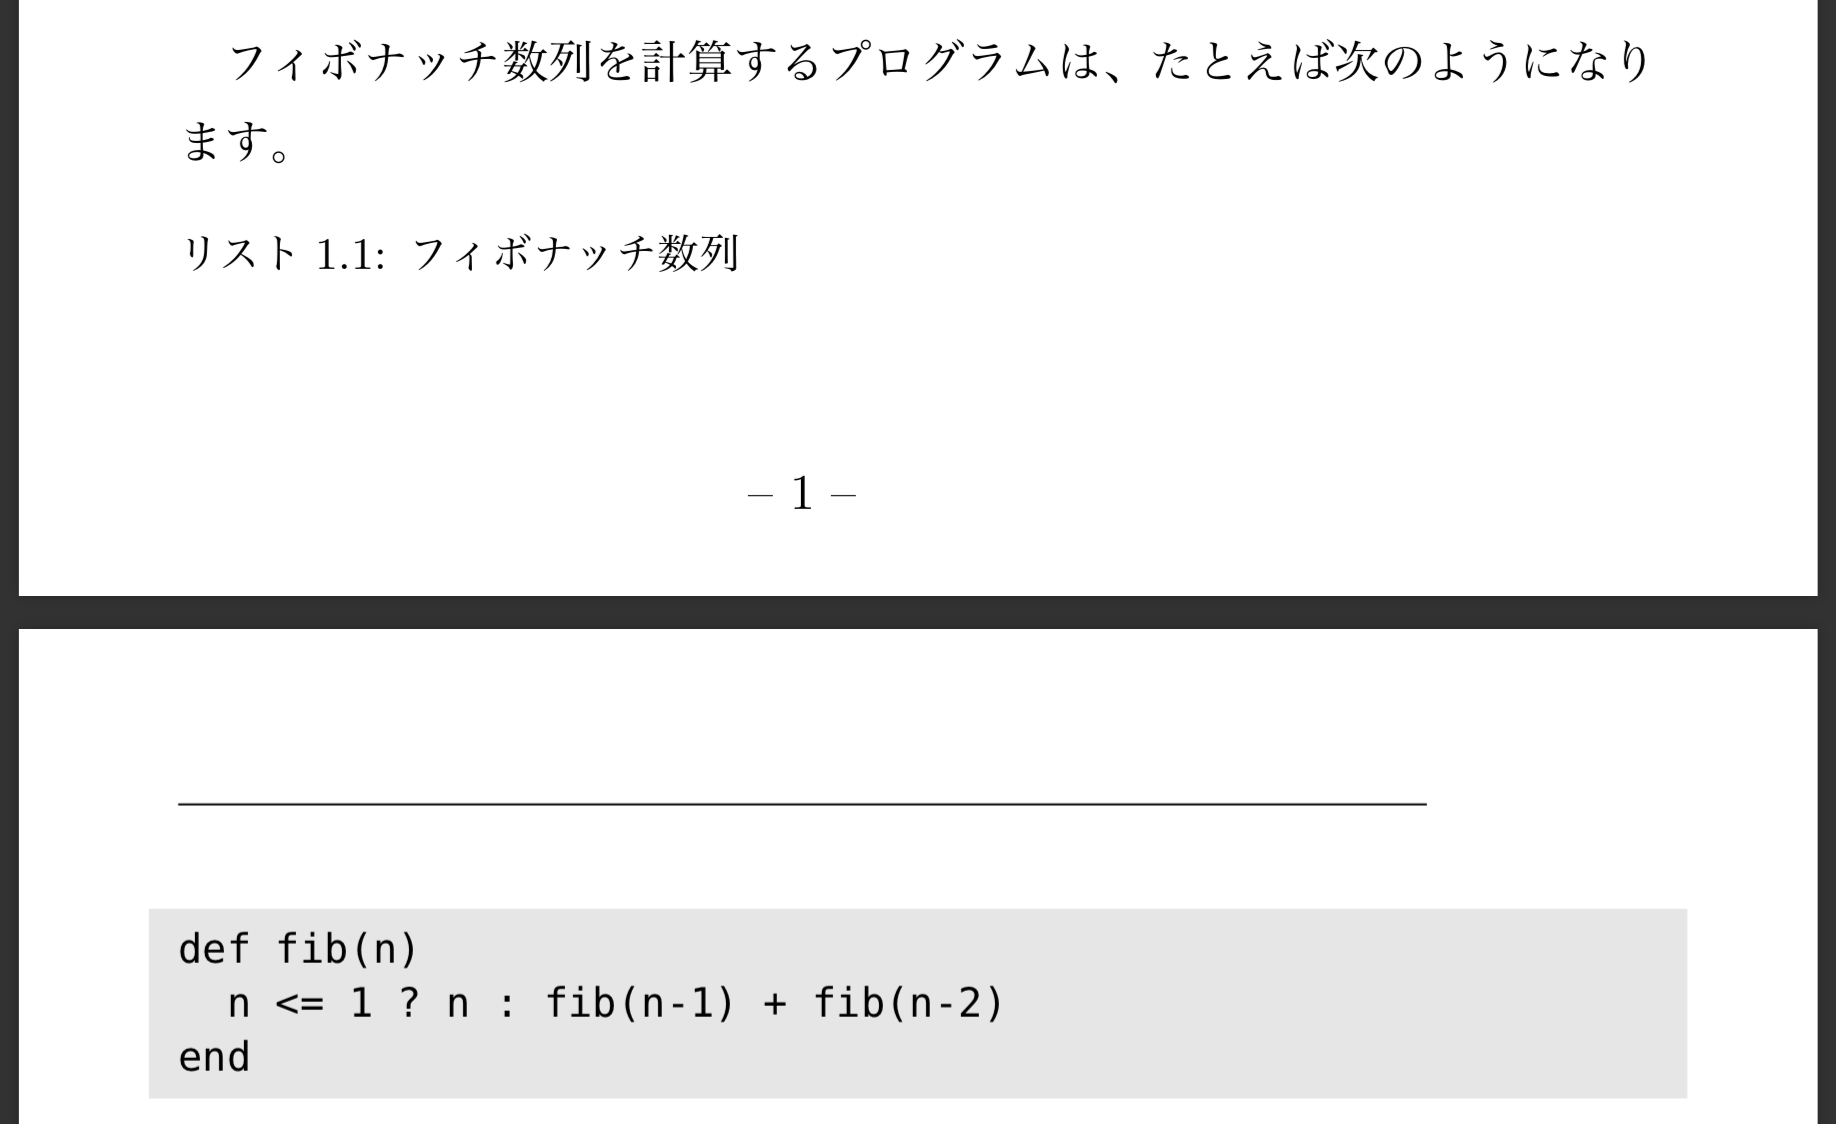
\includegraphics[width=0.8\maxwidth]{./images/chap01-starter/caption_pagebreak.png}%
\reviewimagecaption{キャプションの直後で改ページされた例}
\label{image:chap01-starter:caption_pagebreak}
\end{reviewimage}

Starterではこれを改善し、キャプションの直後では改ページを起こさないようにしました\footnote{これは\LaTeX{}の\reviewem{needspace.sty}で実現しています。}。
かわりにキャプションの直前で改ページされます。

ただし同じページに脚注が複数行あると、判定を間違えてキャプション直後に改ページされることがあります。
これは現在の制限事項です。
経験則として、キャプションの前の文章を増やすとなぜか治ることが多いです。

\subsection*{コラム内の脚注}
\addcontentsline{toc}{subsection}{コラム内の脚注}
\label{sec:1-1-12}

Re:VIEWでは、コラムの中に書いた脚注が消えることがあります。
たとえば次のように書いた場合は、脚注が消えます。

\startercodeblockcaption{コラム内の脚注が消えるサンプル}
\begin{starterprogram}\seqsplit{==[column] サンプル
本文本文\texttt{@}\textless{}fn\textgreater{}\{xxx1\}本文本文。

//footnote[xxx1][脚注脚注脚注。]}\end{starterprogram}

こうではなく、次のようにコラムを明示的に閉じてから脚注を書くと、消えずに表示されます。

\startercodeblockcaption{コラム内の脚注が消えないサンプル}
\begin{starterprogram}\seqsplit{==[column] サンプル
本文本文\texttt{@}\textless{}fn\textgreater{}\{xxx1\}本文本文。

\bfseries{}==[/column]\mdseries{}

//footnote[xxx1][脚注脚注脚注。]}\end{starterprogram}

Starterではこの問題に対処するために、前者のように書かれた場合でも、後者のように自動変換します。

変換はスクリプト\reviewem{lib/hooks/beforetexcompile.rb}が行います。
設定ファイルである\reviewem{config.yml}に「\texttt{hook\textunderscore{}beforetexcompile: [lib/hooks/beforetexcompile.rb]}」という設定を追加しているため、\LaTeX{}コマンドでコンパイルされる前にこのスクリプトが実行されるようになっています。

\subsection*{右寄せ、左寄せ、センタリング}
\addcontentsline{toc}{subsection}{右寄せ、左寄せ、センタリング}
\label{sec:1-1-13}

Starterでは、右寄せや左寄せやセンタリングをする機能を追加しました。

\startercodeblockcaption{サンプル}
\begin{starterprogram}\seqsplit{//textright\{
右寄せのサンプル
//\}
//textleft\{
左寄せのサンプル
//\}
//textcenter\{
センタリングのサンプル
//\}}\end{starterprogram}
\noindent
\reviewem{表示結果:}

\starterresult
\begin{flushright}
右寄せのサンプル
\end{flushright}
\begin{flushleft}
左寄せのサンプル
\end{flushleft}
\begin{center}
センタリングのサンプル
\end{center}
\endstarterresult

しかし、実はRe:VIEWにも右寄せとセンタリングの機能があることが判明しました。
今後はこちらを使うのがいいでしょう\footnote{ただし\url{https://github.com/kmuto/review/blob/master/doc/format.ja.md}には載ってないので、undocumentedな機能です。将来は変更されるかもしれません。}。

\startercodeblockcaption{サンプル}
\begin{starterprogram}\seqsplit{//flushright\{
右寄せのサンプル
//\}
//centering\{
センタリングのサンプル
//\}}\end{starterprogram}
\noindent
\reviewem{表示結果:}

\starterresult

\begin{flushright}
右寄せのサンプル
\end{flushright}

\begin{center}
センタリングのサンプル
\end{center}

\endstarterresult

\subsection*{章の概要}
\addcontentsline{toc}{subsection}{章の概要}
\label{sec:1-1-14}

Starterでは、章(Chapter)の概要を表す「\texttt{//abstract\{} ... \texttt{//\}}」を用意しています。

\startercodeblockcaption{サンプル}
\begin{starterprogram}\seqsplit{//abstract\{
この章では、XXXのXXXという機能について説明します。
この機能を理解することで、あとの章が理解できるようになります。
//\}}\end{starterprogram}
\noindent
\reviewem{表示結果:}

\starterresult
\begin{starterabstract}
この章では、XXXのXXXという機能について説明します。
この機能を理解することで、あとの章が理解できるようになります。
\end{starterabstract}
\endstarterresult

本文と違う見た目にするために、デフォルトでは左右に全角2.5文字文の余白を追加し、かつゴシック体で表示します。
デザインを変更する場合は、\reviewem{sty/starter.sty}で「\texttt{\reviewbackslash{}newenvironment\{starterabstract\}}」を探し、変更してください。

なおこれとよく似た機能として、Re:VIEWには導入文(リード文)を表す「\texttt{//lead\{} ... \texttt{//\}}」が標準で用意されています。
これは主に、詩や物語や聖書からの引用を表すのに使うようです(海外の本にはよくありますよね)。
そのため、「\texttt{//lead}」は\LaTeX{}での引用を表す「\texttt{quotation}」環境に変換されます。

\startercodeblockcaption{サンプル}
\begin{starterprogram}\seqsplit{//lead\{
土に根を下ろし 風と共に生きよう

種と共に冬を越え 鳥と共に春を歌おう
//\}}\end{starterprogram}
\noindent
\reviewem{表示結果:}

\starterresult
\begin{starterlead}
土に根を下ろし 風と共に生きよう

種と共に冬を越え 鳥と共に春を歌おう
\end{starterlead}
\endstarterresult

\subsection*{図が次のページに送られるときにスペースを空けない}
\addcontentsline{toc}{subsection}{図が次のページに送られるときにスペースを空けない}
\label{sec:1-1-15}

Re:VIEWのデフォルトでは、図を入れるときに現在位置に入りきれない場合は、次のページに送られます。
それは仕方ないのですが、このとき現在位置に大きな空きができてしまいます(\reviewimageref{1.2}{image:chap01-starter:figure_heretop}の上)。

\begin{reviewimage}%%figure_heretop
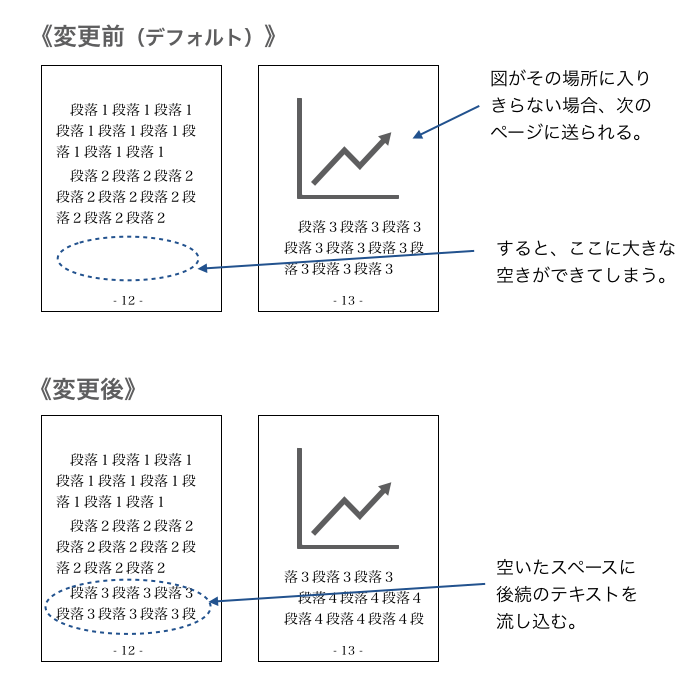
\includegraphics[width=0.8\maxwidth]{./images/chap01-starter/figure_heretop.png}%
\reviewimagecaption{図が次のページに送られると、そこに大きな空きができてしまう}
\label{image:chap01-starter:figure_heretop}
\end{reviewimage}

これに対する解決策として、Starterでは空いたスペースに後続のテキストを流し込む選択肢を用意しています(\reviewimageref{1.2}{image:chap01-starter:figure_heretop}の下)。

そのためには、Starterのプロジェクト作成ページに「画像が現在位置に入りきらず次のページに回されるとき、大きなスペースを空けない (かわりに後続のテキストを流し込む)」というチェックボックスがあるので、これを選んでください。
または、\reviewem{config{-}starter.yml}で「\texttt{image\textunderscore{}position:}」というオプションに「\texttt{h}」を指定してください。

またStarterでは「\texttt{//image}」コマンドを拡張し、図の挿入位置が指定できるようになっています\footnote{実装方法は\reviewem{lib/hooks/monkeypatch.rb}を見てください。}。
これを指定することで、空いたスペースに後続のテキストを流し込むかどうかを、画像ごとに制御できます。

\begin{starteritemize}
\item 「\texttt{//image[][][}\reviewstrong{pos=H}\texttt{]}」なら後続のテキストを流し込まない\\{}
   (つまり画像を現在位置に強制的に配置する)
\item 「\texttt{//image[][][}\reviewstrong{pos=h}\texttt{]}」なら後続のテキストを流し込む\\{}
   (つまり画像が現在位置に入りきらなければ次のページの先頭に配置する)
\end{starteritemize}

画像の倍率も指定する場合は、「\texttt{//image[][][scale=0.5,pos=H]}」のように指定してください。

\begin{starternote}{ページ下部にも画像を配置する}
\begin{starternoteinner}

「\texttt{pos=H}」や「\texttt{pos=h}」のどちらを選んでも、入りきらない画像は次ページに送られます。
そのため、どうしても画像はページ上部に配置されることが多くなり、逆にページ下部には配置されにくくなります。

このバランスの悪さが気になる場合は、(小さい画像を除いて大きめの画像に)「\texttt{pos=bt}」を指定してみてください。
ここで「\texttt{b}」はボトム(bottom)、「\texttt{t}」はトップ(top)を表します。
つまり、まずページ下部に配置を試み、入らないなら次ページ上部に配置します。
これで、全体的に図がページの上部と下部の両方に配置されるはずです。

\end{starternoteinner}
\end{starternote}
\begin{starternote}{「次の図」や「以下の図」という表現を止める}
\begin{starternoteinner}

すでに説明したように、画像の配置場所として「\texttt{pos=H}」\reviewstrong{以外}を指定した場合は、後続のテキストが現在位置に流し込まれます。
そのため、文章中で「次の図は〜」とか「以下の図では〜」と書いていると、図が次ページに配置された場合、読者が混乱します。

このような事態を避けるために、「次の図は〜」や「以下の図では〜」という表現を止めて、「図1.1では〜」のように番号で参照するようにしましょう。
面倒でしょうが、仕方がありません。慣れてください。

\end{starternoteinner}
\end{starternote}

\subsection*{図のまわりを線で囲む}
\addcontentsline{toc}{subsection}{図のまわりを線で囲む}
\label{sec:1-1-16}

Starterでは、図のまわりをグレーの線で囲むことができます。
そのためには「\texttt{//image}」の第3引数に「\texttt{border=on}」を指定します。

\startercodeblockcaption{サンプル}
\begin{starterprogram}\seqsplit{//image[tw{-}icon][デフォルトの表示][scale=0.5,pos=H]

//image[tw{-}icon][まわりを線で囲む][scale=0.5,pos=H,\bfseries{}border=on\mdseries{}]}\end{starterprogram}
\noindent
\reviewem{表示結果:}

\starterresult
\begin{reviewimage}[H]%%tw-icon

\includegraphics[width=0.5\maxwidth]{./images/chap01-starter/tw-icon.jpg}%
\reviewimagecaption{デフォルトの表示}
\label{image:chap01-starter:tw-icon}
\end{reviewimage}
\begin{reviewimage}[H]%%tw-icon
\starterimageframe{%

\includegraphics[width=0.5\maxwidth]{./images/chap01-starter/tw-icon.jpg}%
}%
\reviewimagecaption{まわりを線で囲む}
\label{image:chap01-starter:tw-icon}
\end{reviewimage}
\endstarterresult

\subsection*{何もしない命令「\texttt{@}\textless{}nop\textgreater{}\{...\}」}
\addcontentsline{toc}{subsection}{何もしない命令「\texttt{@}\textless{}nop\textgreater{}\{...\}」}
\label{sec:1-1-17}

Re:VIEWでは、「\texttt{//list\{} ... \texttt{//\}}」や「\texttt{//emlist\{} ... \texttt{//\}}」のようなブロック命令の中で、「\texttt{@\textless{}b\textgreater{}\{}...\texttt{\}}」などのインライン命令が利用できます。
そのため、「\texttt{//emlist\{} ... \texttt{//\}}」の中で「\texttt{@\textless{}b\textgreater{}\{}...\texttt{\}}」そのものを表示させるには次のようなトリックが必要です。

\startercodeblockcaption{サンプル}
\begin{starterprogram}\seqsplit{//emlist\{
  @\textless{}b\textgreater{}\{ABC\}
  @\textless{}code\textgreater{}\textdollar{}@\textdollar{}\textless{}b\textgreater{}\{ABC\}
//\}}\end{starterprogram}
\noindent
\reviewem{表示結果:}

\starterresult
\begin{starterprogram}\seqsplit{  \bfseries{}ABC\mdseries{}
  \texttt{@}\textless{}b\textgreater{}\{ABC\}}\end{starterprogram}
\endstarterresult

つまり「\texttt{@\textless{}b\textgreater{}\{}...\texttt{\}}」のうち「\texttt{@}」だけを「\texttt{@\textless{}code\textgreater{}\{}...\texttt{\}}」で囲うわけです。

この方法はうまく動作しますが、そもそもソースコードを表示するための「\texttt{//emlist\{} ... \texttt{//\}}」の中で「\texttt{@\textless{}code\textgreater{}\{}...\texttt{\}}」を使うのもおかしな話です。

そこでStarterでは、何もしないインライン命令「\texttt{@\textless{}nop\textgreater{}\{}...\texttt{\}}」を用意しました(「nop」は「No Operation」の略です)。
これを使うと、引数を何も加工せず表示します。

サンプルを見てみましょう。

\startercodeblockcaption{サンプル}
\begin{starterprogram}\seqsplit{//emlist\{
1. @\textless{}b\textgreater{}\{ABC\}
2. @\textless{}nop\textgreater{}\textdollar{}@\textless{}b\textgreater{}\{ABC\}\textdollar{}
3. @\textless{}nop\textgreater{}\textdollar{}@\textdollar{}\textless{}b\textgreater{}\{ABC\}
//\}}\end{starterprogram}
\noindent
\reviewem{表示結果:}

\starterresult
\begin{starterprogram}\seqsplit{1. \bfseries{}ABC\mdseries{}
2. @\textless{}b\textgreater{}\{ABC\}
3. @\textless{}b\textgreater{}\{ABC\}}\end{starterprogram}
\endstarterresult

1番目は、「\texttt{ABC}」が太字で表示されてしまいます。
今は「\texttt{@\textless{}b\textgreater{}\{ABC\}}」と表示したいので、これは意図とは違います。

2番目は、「\texttt{@\textless{}b\textgreater{}ABC}」と表示されました(波カッコの「\texttt{\{}」と「\texttt{\}}」が消えています)。
実は\LaTeX{}に変換された段階では「\texttt{@\textless{}b\textgreater{}\{ABC\}}」となっていますが、\LaTeX{}では波カッコが特別な意味を持つため、「\texttt{@\textless{}b\textgreater{}\{ABC\}}」ではなく「\texttt{@\textless{}b\textgreater{}ABC}」と表示されてしまいます。

3番目は、「\texttt{@\textless{}b\textgreater{}\{ABC\}}」と表示されました。
これが期待した出力です。
2番目との違いは、「\texttt{@}\texttt{\textless{}nop\textgreater{}\textdollar{}}...\texttt{\textdollar{}}」の引数に「\texttt{\{}」と「\texttt{\}}」を含めなかったことです。
これによって、\LaTeX{}へ変換するときに「\texttt{\{}」と「\texttt{\}}」が適切にエスケープされます。

このような落とし穴はありますが、ブロック命令の中でインライン命令そのものを表示したい場合は、「\texttt{@\textless{}nop\textgreater{}\{}...\texttt{\}}」を使ってください。

なお「\texttt{@\textless{}nop\textgreater{}\{\}}」はもともと「\texttt{@\textless{}letitgo\textgreater{}\{\}}」という名前でしたが、長すぎるという意見があったので「\texttt{@\textless{}nop\textgreater{}\{\}}」になりました。後方互換性のため、「\texttt{@\textless{}letitgo\textgreater{}\{\}}」も使えます。

\subsection*{章や項を参照する「\texttt{@}\texttt{\textless{}secref\textgreater{}\{\}}」}
\addcontentsline{toc}{subsection}{章や項を参照する「\texttt{@}\texttt{\textless{}secref\textgreater{}\{\}}」}
\label{sec:1-1-18}

Re:VIEWでは、「\texttt{@}\texttt{\textless{}hd\textgreater{}\{\}}」を使って節(Section)や項(Subsection)を参照できます。
しかしこの機能には問題点があります。

\begin{starteritemize}
\item Re:VIEWのデフォルト設定\footnote{Re:VIEWのデフォルトでは\reviewem{config.yml}で「\texttt{secnolevel: 2}」と設定されています。これが3以上でないと、項(Subsection)に番号がつきません。}では、章(Chapter)と節(Section)には番号がつくけど、項(Subsection)には番号がつかない。
\item そのため、「\reviewem{@\textless{}hd\textgreater{}\{\}}」で項(Subsection)を参照すると、番号がなくて項タイトルだけになるので文章がとても不自然になる。
\end{starteritemize}

サンプルを使って説明しましょう。
たとえば次のような原稿ファイルがあったとします。

\startercodeblockcaption{ファイル:chap{-}pattern.re}
\begin{starterprogram}\seqsplit{= デザインパターンの紹介

==\{sec{-}visitor\} Visitorパターン

===\{subsec{-}motivation\} 動機

===\{subsec{-}structure\} 構造

===\{subsec{-}impl\} 実装例
}\end{starterprogram}

文章の構造は次のようになっていますね。

\begin{starteritemize}
\item 「デザインパターンの紹介」は章(Chapter)

\begin{starteritemize}
\item 「Visitorパターン」は節(Section)

\begin{starteritemize}
\item 「動機」と「構造」と「実装例」は項(Subsection)
\end{starteritemize}

\end{starteritemize}

\end{starteritemize}

さてRe:VIEWのデフォルト設定のままだと、次のように章と節には番号がつくけど、項には番号がつきません。

\vspace*{\baselineskip}
\noindent
\reviewem{表示例:}

\starterresult
\vspace*{\baselineskip}
\par\noindent
{\LARGE\headfont 第1章 デザインパターンの紹介}
\bigskip
\par\noindent
{\Large\headfont 1.1 Visitorパターン}
\bigskip
\par\noindent
{\large\headfont 動機}
\bigskip
\par\noindent
{\large\headfont  構造}
\bigskip
\par\noindent
{\large\headfont  実装例}
\par
\vspace*{\baselineskip}
\endstarterresult

このことを踏まえたうえで、節や項を「\texttt{@}\texttt{\textless{}hd\textgreater{}\{\}}」で参照するとどう表示されるでしょうか。

\begin{starteritemize}
\item 節(Section)には番号がついているので、たとえば「\texttt{@}\texttt{\textless{}hd\textgreater{}\{sec{-}visitor\}}」のように節を参照すると、「1.1 Visitorパターン」のように表示されます。
   これだと番号がついているので、読者は節を探しやすいです。
\item しかし項(Subsection)には番号がついていないので、たとえば「\texttt{@}\texttt{\textless{}hd\textgreater{}\{subsec{-}motivation\}}」や「\texttt{@}\texttt{\textless{}hd\textgreater{}\{subsec{-}structure\}}」のように項を参照すると、「動機」や「構造」とだけ表示されてしまいます。
   これだと番号がついていないので、読者は項を探せないでしょう。
\end{starteritemize}

\startercodeblockcaption{サンプル(最初の1つは節を参照、残り3つは項を参照)}
\begin{starterprogram}\seqsplit{ * @\textless{}hd\textgreater{}\{sec{-}visitor\}
 * @\textless{}hd\textgreater{}\{subsec{-}motivation\}
 * @\textless{}hd\textgreater{}\{subsec{-}structure\}
 * @\textless{}hd\textgreater{}\{subsec{-}impl\}}\end{starterprogram}
\noindent
\reviewem{表示結果:}

\starterresult

\begin{starteritemize}
\item 「1.1 Visitorパターン」
\item 「動機」
\item 「構造」
\item 「実装例」
\end{starteritemize}

\endstarterresult

問題点をもう一度整理しましょう。

\begin{starteritemize}
\item Re:VIEWのデフォルト設定では、項(Subsection)に番号がつかない。
\item そのため、「\texttt{@}\texttt{\textless{}hd\textgreater{}\{\}}」で項を参照するとタイトルだけになってしまい、番号がつかないので読者が項を探せない。
\end{starteritemize}

この問題に対し、Starterでは「\texttt{@}\texttt{\textless{}secref\textgreater{}\{\}}」という新しい命令を用意しました。
この新命令には次のような利点があります。

\begin{starteritemize}
\item 番号のついていない項でも、親となる節を使うことで探しやすい表示をしてくれる。
\item その項のページ番号がつくので、該当ページに直接アクセスできる。
\end{starteritemize}

次のサンプルを見れば、「\texttt{@}\texttt{\textless{}hd\textgreater{}\{\}}」との違いがすぐに分かるでしょう。

\startercodeblockcaption{サンプル(最初の1つは節を参照、残り3つは項を参照)}
\begin{starterprogram}\seqsplit{ * \bfseries{}@\mdseries{}\bfseries{}\textless{}secref\textgreater{}\mdseries{}\{sec{-}visitor\}
 * \bfseries{}@\mdseries{}\bfseries{}\textless{}secref\textgreater{}\mdseries{}\{subsec{-}motivation\}
 * \bfseries{}@\mdseries{}\bfseries{}\textless{}secref\textgreater{}\mdseries{}\{subsec{-}structure\}
 * \bfseries{}@\mdseries{}\bfseries{}\textless{}secref\textgreater{}\mdseries{}\{subsec{-}impl\}}\end{starterprogram}
\noindent
\reviewem{表示結果:}

\starterresult

\begin{starteritemize}
\item 「1.1 Visitorパターン」(p.1)
\item 「1.1 Visitorパターン」内の「動機」(p.1)
\item 「1.1 Visitorパターン」内の「構造」(p.1)
\item 「1.1 Visitorパターン」内の「実装例」(p.1)
\end{starteritemize}

\endstarterresult

これを見ると、番号がついていない項の前に番号がついている節が置かれていること、またページ番号がついていることが分かります。
どちらも\texttt{@}\texttt{\textless{}hd\textgreater{}\{\}}にはない特徴であり、\texttt{@}\texttt{\textless{}hd\textgreater{}\{\}}で参照するより節や項が探しやすくなります。

その他の注意事項です。

\begin{starteritemize}
\item 「\texttt{@}\texttt{\textless{}secref\textgreater{}\{\}}」は、節でも項でも、あるいは目(Subsubsection)でも参照できます。
   今まで「\texttt{@}\texttt{\textless{}hd\textgreater{}\{\}}」を使っていた箇所はすべて「\texttt{@}\texttt{\textless{}secref\textgreater{}\{\}}」で置き換えられます。
   ただし、章(Chapter)は参照できないので、その場合は「\texttt{@}\texttt{\textless{}chapref\textgreater{}\{\}}」を使ってください。
\item 項にも番号をつけるよう設定している場合は、「\texttt{@}\texttt{\textless{}secref\textgreater{}\{\}}」の表示結果は「\texttt{@}\texttt{\textless{}hd\textgreater{}\{\}}」にページ番号をつけたものと同じです。
\item 他の章(Chapter)の節や項を参照する場合は、たとえば\\{}
  「\texttt{@}\texttt{\textless{}secref\textgreater{}\{chap{-}pattern\textbar{}sec{-}visitor\}}」や\\{}
  「\texttt{@}\texttt{\textless{}secref\textgreater{}\{chap{-}pattern\textbar{}subsec{-}impl\}}」のように書いてください。わざわざ\\{}
  「\texttt{@}\texttt{\textless{}secref\textgreater{}\{chap{-}pattern\textbar{}sec{-}visitor\textbar{}subsec{-}impl\}}」のように書く必要はありません。
\end{starteritemize}

\subsection*{「\reviewem{@}\reviewem{\textless{}chapref\textgreater{}\{\}}」や「\reviewem{@}\reviewem{\textless{}hd\textgreater{}\{\}}」をリンクに}
\addcontentsline{toc}{subsection}{「\reviewem{@}\reviewem{\textless{}chapref\textgreater{}\{\}}」や「\reviewem{@}\reviewem{\textless{}hd\textgreater{}\{\}}」をリンクに}
\label{sec:1-1-19}

Starterでは、「@\textless{}chapref\textgreater{}\{\}」や「@\textless{}hd\textgreater{}\{\}」がリンクになるように設定しています。
そのために次のような設定をしています。

\begin{starteritemize}
\item \reviewem{config.yml}に「\texttt{chapterlink: true}」という設定を追加(最終行)。
\item \reviewem{sty/starter.sty}で「\reviewem{\reviewbackslash{}reviewsecref}」を再定義し、「\reviewem{\reviewbackslash{}hyperref}」を使うように変更。
\end{starteritemize}

\startercodeblockcaption{リスト:\reviewbackslash{}reviewsecrefを再定義}
\begin{starterprogram}\seqsplit{\reviewbackslash{}renewcommand\{\reviewbackslash{}reviewsecref\}[2]\{\%
  \reviewbackslash{}hyperref[\#2]\{\#1\}(p.\reviewbackslash{}pageref\{\#2\})\%     \% 節や項のタイトルがリンク
  \%\{\#1\}(\reviewbackslash{}hyperref[\#2]\{p.\reviewbackslash{}pageref\{\#2\}\})\%  \% ページ番号がリンク
\}}\end{starterprogram}

これらはRe:VIEWに実装済みの機能であり、Starterはそれらを有効化しただけです。
しかしこれらの機能はRe:VIEWのドキュメントには書かれていないので、もしかしたら将来的に変更されるかもしれません。

またStarterの追加機能である「\reviewem{@}\reviewem{\textless{}secref\textgreater{}\{\}}」でも、リンクが作成されます。

\subsection*{ターミナルでのカーソル}
\addcontentsline{toc}{subsection}{ターミナルでのカーソル}
\label{sec:1-1-20}

ターミナルでのカーソルを表す機能を用意しました。
たとえば次の例では、2行目の真ん中の「\texttt{f}」にカーソルがあることを表しています。

\startercodeblockcaption{カーソル}
\label{}
\begin{starterterminal}\seqsplit{function fib(n) \{
  return n \textless{}= 1 ? n : {\startercursor{f}}ib(n{-}1) : fib(n{-}2);
\}
\textasciitilde{}
\textasciitilde{}
"fib.js" 3L, 74C written}\end{starterterminal}

\subsection*{その他}
\addcontentsline{toc}{subsection}{その他}
\label{sec:1-1-21}

\begin{starteritemize}
\item ブロック命令「\texttt{//clearpage}」で改ページします。
   また過去との互換性のために、インライン命令「\texttt{@\textless{}clearpage\textgreater{}\{\}}」も使えます。
\item 「\texttt{@\textless{}hearts\textgreater{}\{\}}」とすると、「$\heartsuit$」と表示されます。
\item 「\texttt{@\textless{}TeX\textgreater{}\{\}}」とすると、「\TeX{}」と表示されます。
\item 「\texttt{@\textless{}LaTeX\textgreater{}\{\}}」とすると、「\LaTeX{}」と表示されます。
\end{starteritemize}

\section{レイアウトやデザインに関する変更や拡張}
\label{sec:1-2}
\label{sec-design}

\subsection*{Starterの設定ファイル「\reviewem{config{-}starter.yml}」}
\addcontentsline{toc}{subsection}{Starterの設定ファイル「\reviewem{config{-}starter.yml}」}
\label{sec:1-2-1}

Starterでは、「\reviewem{config{-}starter.yml}」という設定ファイルを新たに用意しました。
この設定ファイルを編集することで、プロジェクトをダウンロードしたあとでもレイアウトやデザインを簡単に変更できます。

たとえば以下のことが変更できます。

\begin{starteritemize}
\item PDFのターゲット(印刷用か、ダウンロード用か)
\item 章や節や項のデザイン
\item プログラムやターミナルの表示で使う等幅フォント
\item ドラフトモード(画像を枠線だけで表示する)
\end{starteritemize}

残念ながら、プロジェクト作成時にGUIで設定できたことがすべて「\reviewem{config{-}starter.yml}」でできるわけではありません。しかしなるべく多くのことがこの設定ファイルで変更できるようにするつもりです。

\subsection*{フォントサイズの変更に対応}
\addcontentsline{toc}{subsection}{フォントサイズの変更に対応}
\label{sec:1-2-2}

Re:VIEW 2.5は、標準では本文のフォントサイズを9ptや8ptに指定しても、効いてくれません(まじかー!)。
ウソだと思うかも知れませんが、実際に苦しんだ人の証言\footnote{\url{https://www.slideshare.net/KazutoshiKashimoto/nagoya0927-release}のp.21とp.22。}があるのでご覧ください。
先人の苦労が偲ばれます。

\begin{reviewimage}%%slide2
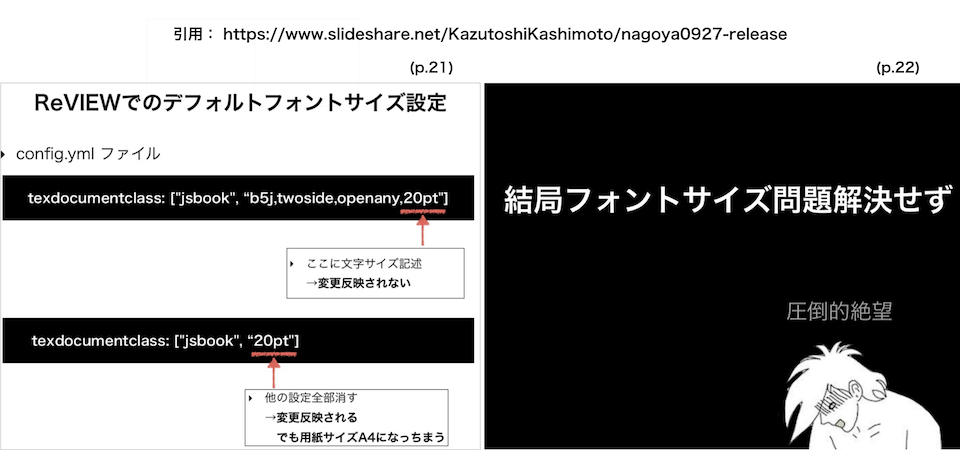
\includegraphics[width=\maxwidth]{./images/chap01-starter/slide2.png}%
\reviewimagecaption{フォントやページサイズを変更できなかった人の証言}
\label{image:chap01-starter:slide2}
\end{reviewimage}

この問題は、「\reviewem{geometry.sty}」というスタイルファイルをオプションなしで読み込んでいることが原因です\footnote{簡単に書いてますけど、原因が\reviewem{geometry.sty}であることを突き止めるのには大変な時間がかかり、正月休みを潰してしまいました。コノウラミハラサデオクベキカ!}。
Starterではこれを読み込まないように修正している\footnote{修正箇所は、\reviewem{layouts/layout.tex.erb}の50行目あたりです。}ため、フォントサイズを9ptや8ptに指定すればそのサイズになります。

\subsection*{A5サイズの指定に対応}
\addcontentsline{toc}{subsection}{A5サイズの指定に対応}
\label{sec:1-2-3}

Re:VIEW 2.5は、標準ではA5サイズの指定が効いてくれません(まじかー!)。
ウソだと思うかも知れませんが、実際にトラブルに陥った人の証言があります\footnote{\url{https://blog.vtryo.me/entry/submit-of-journey}}。

\begin{starterquote}

 \\{}
\reviewstrong{トラブル発生!!}\\{}\\{}
原稿データチェック、表紙チェック、ともに問題なく終わったかにみえた午後1時。\\{}
何かに気づいたお姉さんの声音が変わりました。\\{}
「すみません、PDFサイズ……B5になってます」\\{}
「えっ……」\\{}
めのまえがまっくらになった。\\{}
セイチョウ・ジャーニーはA5で制作しているはずなのに、B5サイズに??\\{}
わからない!どうして!だって何度も確認したはずだ!!\\{}
と度重なる徹夜で脳死寸前の僕はパニック状態になりました。\\{}

\end{starterquote}

入稿で明らかになるトラブル!怖いですねー。
こういう予期せぬトラブルがあるので、締切りギリギリまで作業するのは止めて、余裕をもって入稿しましょう。

さて、A5にならない問題は2種類あります。

\begin{starteritemize}
\item 本文の大きさがA5サイズにならない。
\item 本文の大きさはA5なのにPDFがA5サイズにならない。
\end{starteritemize}

前者は、「\reviewem{geometry.sty}」が原因です。
すでに説明したように、Starterでは「\reviewem{geometry.sty}」を読み込まないようにしているため、この問題は起こりません。

後者は、上で紹介したトラブルですね。
これは\reviewem{jsbook.sty}のオプションに「\reviewem{papersize}」が指定されてないせいです。
Starterではこのオプションを指定しているので、A5やB5の指定どおりのPDFが生成されます。

詳しくは、\reviewem{config.yml}の「\texttt{texdocumentclass:}」を参照してください。

\startercodeblockcaption{config.yml}
\begin{starterprogram}\seqsplit{texdocumentclass: ["jsbook",
    \#"uplatex,papersize,twoside,b5j,10pt,openright" \# B5 10pt 右起こし
    \#"uplatex,papersize,twoside,b5j,10pt,openany"   \# B5 10pt 両起こし
    \#"uplatex,papersize,twoside,a5j,9pt,openright"  \# A5  9pt 右起こし
    \#"uplatex,papersize,twoside,a5j,9pt,openany"    \# A5  9pt 両起こし
    \#"uplatex,papersize,oneside,a5j,10pt,openany"   \# A5 10pt 両起こし
    "uplatex,papersize,twoside,a5j,9pt,openright"
]}\end{starterprogram}

\subsection*{本文の幅を全角40文字より長くできる}
\addcontentsline{toc}{subsection}{本文の幅を全角40文字より長くできる}
\label{sec:1-2-4}

\LaTeX{}の\reviewem{jsbook.cls}ファイルを使うと、デフォルトでは本文の幅の最大値が40文字までに制限されています。
これは、1行が全角40文字より長いと読みづらくなるからという理由だそうです\footnote{\url{https://oku.edu.mie-u.ac.jp/~okumura/jsclasses/}に、\reviewem{jsbook.cls}の作者である奥村先生が『書籍では1行の長さが全角40文字を超えないようにしています。』と解説しています。}。

そのため、B5サイズだとページ左右の余白が広めになってしまいます。
ページ数を抑えて印刷代を下げたい人にとって、この余白はコストを増加させる要因です。

Starterでは\reviewem{sty/mytextsize.sty}で本文幅を再設定することで、本文の幅を40文字より広くできます。
B5サイズでフォントが10ptだと、1行あたり全角42〜45文字がいいでしょう。

ただしA5サイズ(フォント9pt)では、1行あたり40文字を超えるのはやめたほうがいいです。
参考までに市販の技術書だと、A5サイズで1行あたり全角39文字にすることが多いようです。

\subsection*{奇数ページと偶数ページで左右の余白を変える}
\addcontentsline{toc}{subsection}{奇数ページと偶数ページで左右の余白を変える}
\label{sec:1-2-5}
\label{jwevu}

本文の幅を広げる場合でも、左右の余白はちゃんと取りましょう(\reviewimageref{1.6}{image:chap01-starter:margin_book})。

\begin{reviewimage}%%margin_book
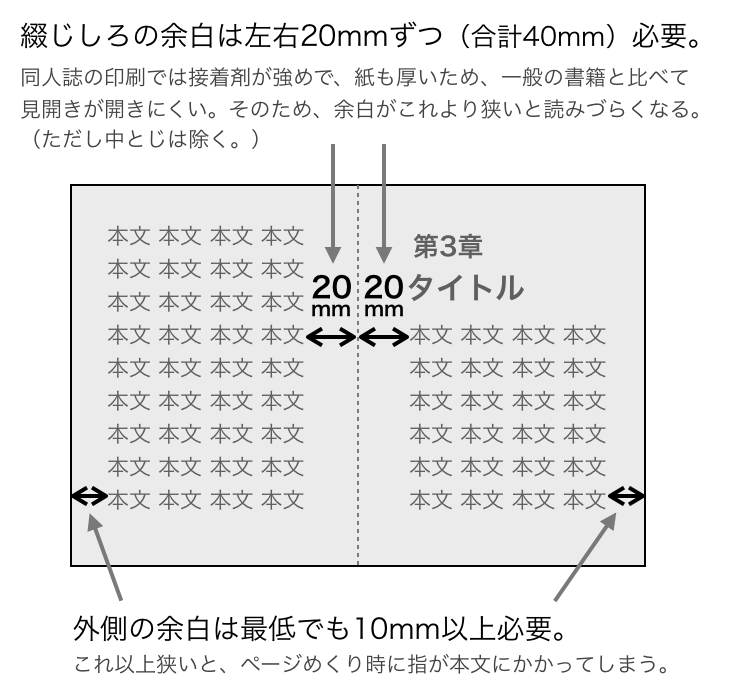
\includegraphics[width=0.7\maxwidth]{./images/chap01-starter/margin_book.png}%
\reviewimagecaption{奇数ページと偶数ページで左右の余白を変える}
\label{image:chap01-starter:margin_book}
\end{reviewimage}

\begin{starteritemize}
\item 本を開いたときの中央(「ノド」という)の余白、つまり左ページの右余白と右ページの左余白は、最低でも2cmは確保しましょう。
   そうしないと、ノド近くの文章がとても読みづらくなります。
\item 本を開いたときの外側(「小口」という)の余白、つまり左ページの左余白と右ページの右余白は、最低でも1cmは確保しましょう。
   そうしないと、ページをめくるときに指が本文にかかってしまい、読みにくいです。
\end{starteritemize}

Starterではこういったことを考慮し、本文の幅を広げる(つまり1行あたりの文字数を増やす)場合には小口側の余白だけを減らすようにしています。
詳しくは\reviewem{sty/mytextsize.sty}を見てください。

\subsection*{ページ上部の余白を減らし、その分を本文の高さに追加}
\addcontentsline{toc}{subsection}{ページ上部の余白を減らし、その分を本文の高さに追加}
\label{sec:1-2-6}

\LaTeX{}の標準のデザインでは、ページ上部の余白が大きめになっています。
ページ数を少しでも減らして印刷代を抑えたい場合は、この余白がとても気になります。

Starterではこの余白を約1cm減らし\footnote{実はjsbook.clsでは「\reviewem{1cm}」は1cmより少し大きく扱われ、厳密に1cmを指定したい場合は「\reviewem{1truecm}」とする必要があります。しかしここではそこまで厳密な1cmを必要とはしていないので、\reviewem{sty/mytextsize.sty}では「\reviewem{1cm}」と指定しています。}、その分を本文の高さに追加しています。
詳しくは\reviewem{sty/mytextsize.sty}を見てください。

\subsection*{ソースコード表示用のフォントを変更}
\addcontentsline{toc}{subsection}{ソースコード表示用のフォントを変更}
\label{sec:1-2-7}

\LaTeX{}のデフォルトでは、装飾が多めのフォントがソースコードの表示に使われています(\reviewimageref{1.7}{image:chap01-starter:font_beramono}の上半分)。
このフォントは「0」と「O」や「1」と「l」の区別がつきにくく、また太字にしてもあまり目立たないという欠点があります。

\begin{reviewimage}%%font_beramono
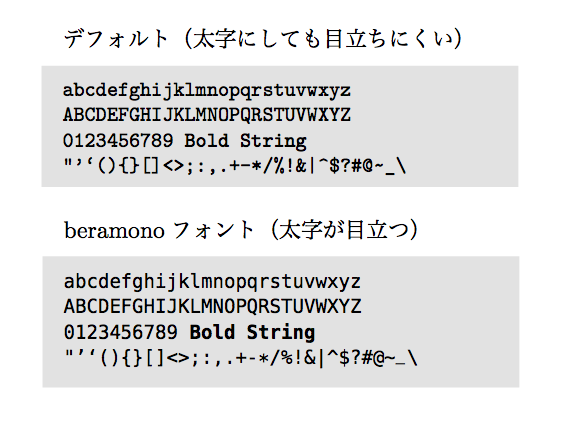
\includegraphics[width=0.7\maxwidth]{./images/chap01-starter/font_beramono.png}%
\reviewimagecaption{ソースコードの表示に使われるフォント}
\label{image:chap01-starter:font_beramono}
\end{reviewimage}

Starterでは、ソースコードの表示に使うフォントを、装飾が少ないもの(Bera Mono\footnote{\url{http://www.tug.dk/FontCatalogue/beramono/} でサンプルが見れます。})に変更しています(\reviewimageref{1.7}{image:chap01-starter:font_beramono}の下半分)。
このフォントは「0」と「O」や「1」と「l」の区別がつきやすく、また太字にしたときも目立つようになっています。
ただし「\texttt{'}」(シングルクォート)と「\texttt{`}」(バッククォート)の区別がつきにくくなっているので注意してください。

ソースコードの表示に向くフォントとしては、他にも「Inconsolata」\footnote{\url{http://www.tug.dk/FontCatalogue/inconsolata/} でサンプルが見れます。}や「Nimbus Mono Narrow」\footnote{\url{http://www.tug.dk/FontCatalogue/nimbus15mononarrow/} でサンプルが見れます。}があります。
興味がある人は調べてみてください。

\subsection*{章や節のデザインを変更可能}
\addcontentsline{toc}{subsection}{章や節のデザインを変更可能}
\label{sec:1-2-8}

Starterでは、章(Chapter)や節(Section)のデザインを変更できます。
例を2つ挙げておきます(\reviewimageref{1.8}{image:chap01-starter:chaphead_design_3}、\reviewimageref{1.9}{image:chap01-starter:chaphead_design_2})。

\begin{reviewimage}%%chaphead_design_3
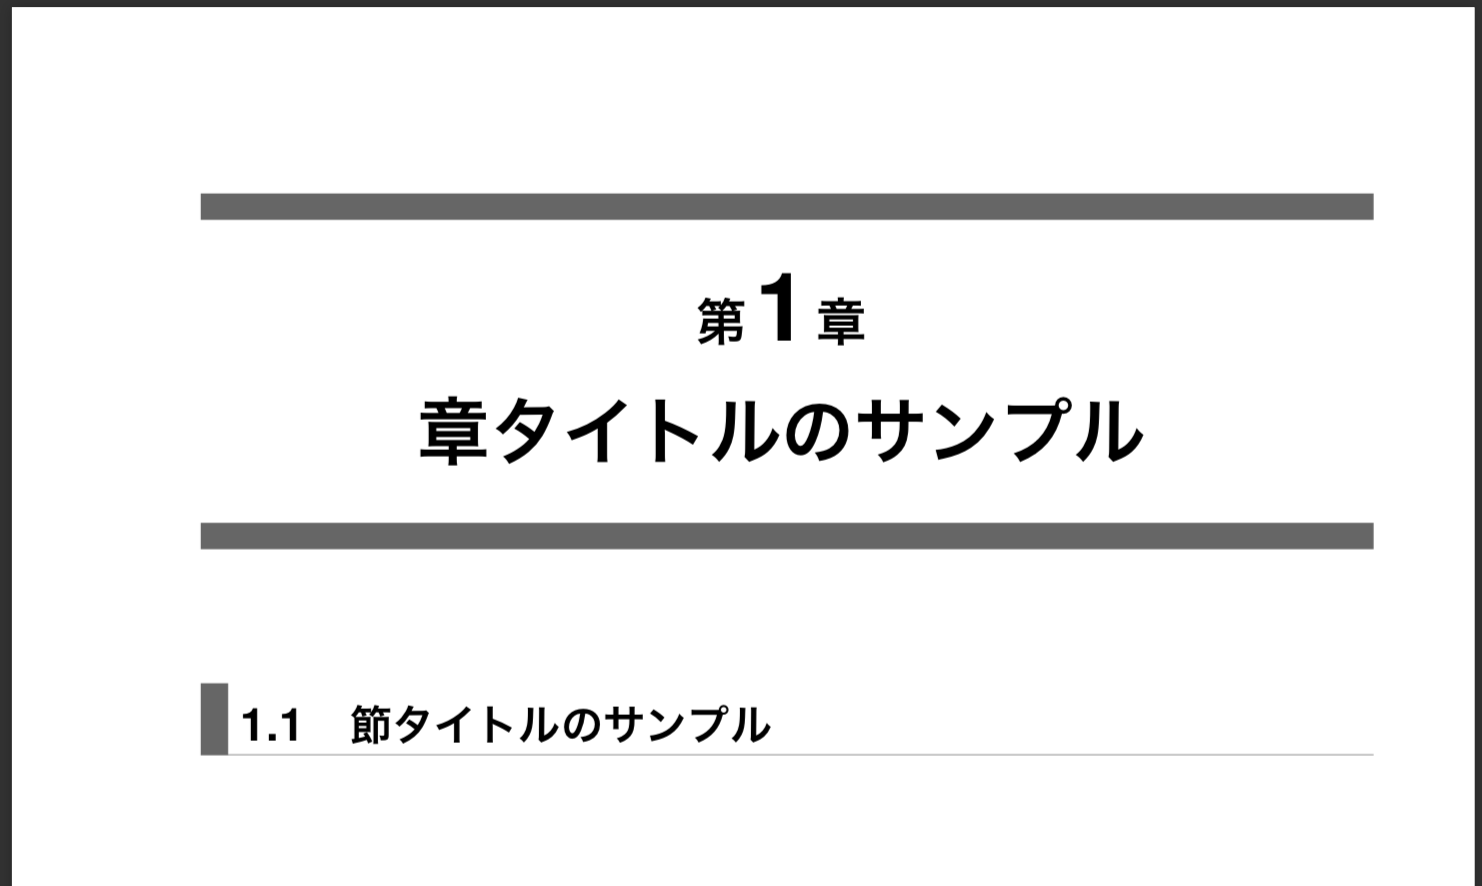
\includegraphics[width=0.7\maxwidth]{./images/chap01-starter/chaphead_design_3.png}%
\reviewimagecaption{章タイトルをセンタリング、上下に太線、節タイトルに下線}
\label{image:chap01-starter:chaphead_design_3}
\end{reviewimage}
\begin{reviewimage}%%chaphead_design_2
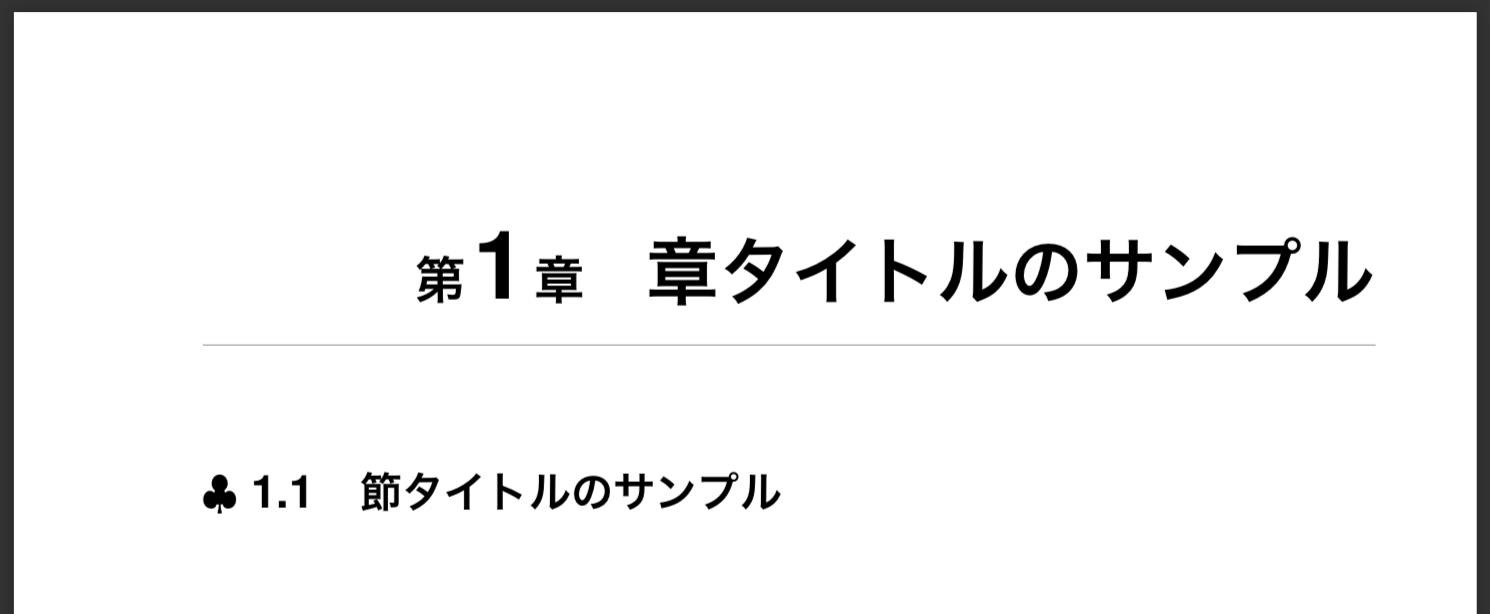
\includegraphics[width=0.7\maxwidth]{./images/chap01-starter/chaphead_design_2.png}%
\reviewimagecaption{章タイトルを右寄せ、下に細線、節タイトルの行頭にクローバー}
\label{image:chap01-starter:chaphead_design_2}
\end{reviewimage}

これらのデザインを調整するときは、\reviewem{config{-}starter.yml}で設定を変更してください。
この設定で飽き足らない場合は\reviewem{sty/starter.sty}を編集してください。

なおStarterでは、\reviewimageref{1.8}{image:chap01-starter:chaphead_design_3}のように章タイトルの上下に太い線を入れた場合でも、まえがきや目次やあとがきのタイトルには太い線を入れないようにしています。
これは意図的な仕様です。

\subsection*{章のタイトルページを作成可能}
\addcontentsline{toc}{subsection}{章のタイトルページを作成可能}
\label{sec:1-2-9}

Starterでは、章(Chapter)のタイトルと概要を独立したページにできます(\reviewimageref{1.10}{image:chap01-starter:chaptitlepage_sample})。
これは商用の書籍ではよく見かける方法です。

\begin{reviewimage}%%chaptitlepage_sample
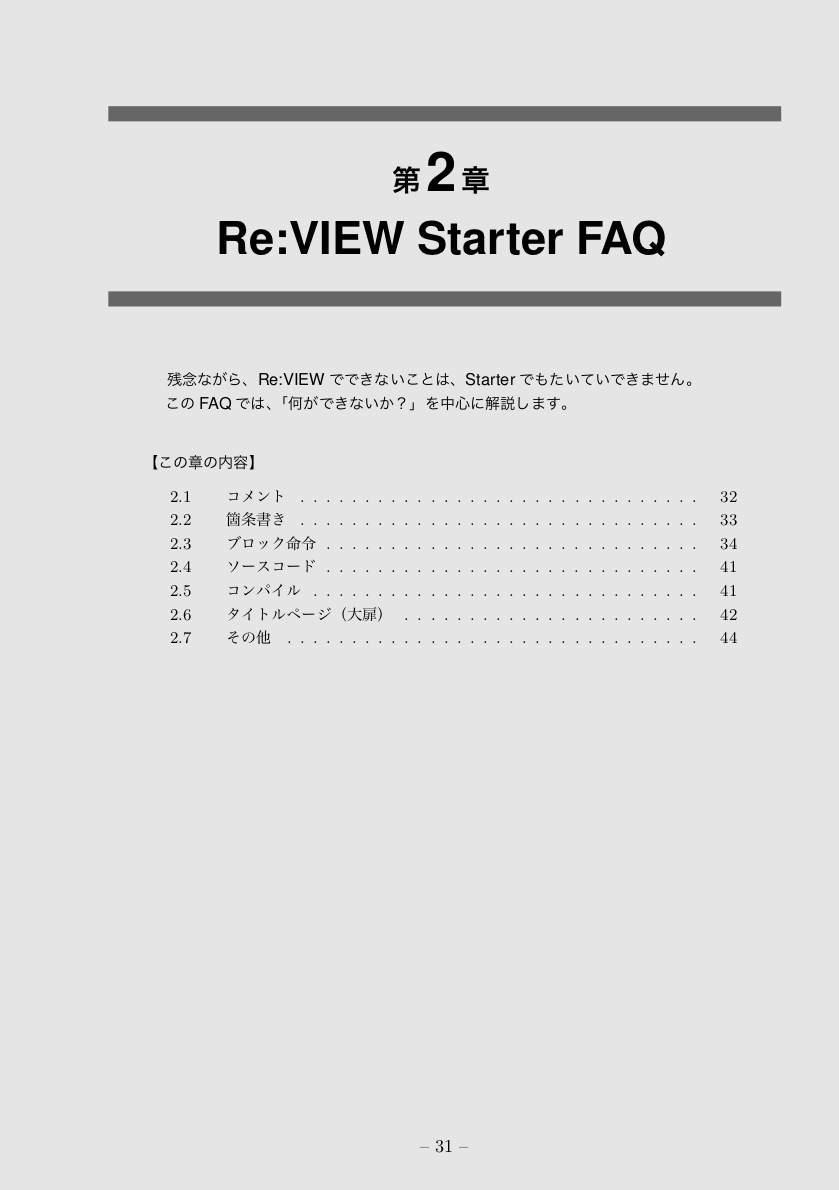
\includegraphics[width=0.5\maxwidth]{./images/chap01-starter/chaptitlepage_sample.png}%
\reviewimagecaption{章のタイトルと概要を独立したページにした例(章ごとの目次つき)}
\label{image:chap01-starter:chaptitlepage_sample}
\end{reviewimage}

やり方は簡単で、章タイトルと概要を書いたあとに「\texttt{//makechaptitlepage[toc=section]}」と書くだけです。
これで章タイトルページが作られ、背景色がつき、その章の目次もつきます\footnote{実装の詳細は\reviewem{sty/starter.sty}の\reviewem{makechaptitlepage}コマンドを参照してください。}。

\startercodeblockcaption{サンプル}
\begin{starterprogram}\seqsplit{= Re:VIEW Starter FAQ

//abstract\{
残念ながら、Re:VIEWでできないことは、Starterでもたいていできません。

このFAQでは、「何ができないか?」を中心に解説します。
//\}

\bfseries{}//makechaptitlepage[toc=section]\mdseries{}}\end{starterprogram}

ただし、「\texttt{//makechaptitlepage[toc=section]}」はすべての章に書く必要があります。
これを書き忘れた章があると、そこだけ章タイトルページが作られません。
注意してください。

\subsection*{目次の文字を小さく、行間を狭く}
\addcontentsline{toc}{subsection}{目次の文字を小さく、行間を狭く}
\label{sec:1-2-10}

Starterでは、目次のデザインを少し変更しています。

\begin{starteritemize}
\item 章(Section)の文字をゴシック体にしました。
   項(Subsection)の文字は明朝体のままなので、これで目次での章と項が見分けやすくなります。
\item 項(Subsection)の文字を少し小さくし、行間を狭くしました。
   これにより、目次にとられるページ数を少しだけ減らせます。
\end{starteritemize}

目次のデザインを修正する場合は、\reviewem{sty/starter.sty}の中で「\reviewem{\reviewbackslash{}l@section}」や「\reviewem{\reviewbackslash{}l@subsection}」を探して、適宜修正してください。
特に目次のページ数が多い場合は、行間を狭めて(「\reviewem{\reviewbackslash{}baselineskip}」を小さくして)みてください。

\subsection*{キャプションのデザインを変更}
\addcontentsline{toc}{subsection}{キャプションのデザインを変更}
\label{sec:1-2-11}

Starterでは、ソースコードや表や図のキャプション(説明)を次のように変更しています。

\begin{starteritemize}
\item フォントをゴシック体にする
\item 先頭に「▲」や「▼」をつける
\end{starteritemize}

これはTechBooster製テンプレートのデザインを参考にしました。
ただし\LaTeX{}マクロの定義はまったく別です\footnote{なおこれに関して、「\texttt{\reviewbackslash{}reviewimagecaption}」というコマンドを新たに定義し、「\texttt{\reviewbackslash{}reviewimage}」環境が「\texttt{\reviewbackslash{}caption}」のかわりにそれを使うよう、LATEXBuilder\#image\textunderscore{}image()にモンキーパッチを適用しています。モンキーパッチはlib/hooks/monkeypatch.rbにあり、review{-}ext.rbが読み込んでいます。}。

\subsection*{引用のデザインを変更}
\addcontentsline{toc}{subsection}{引用のデザインを変更}
\label{sec:1-2-12}

引用「\texttt{//quote\{} ... \texttt{//\}}」のデザインを変更し、左側に縦棒がつくようにしました。

Re:VIEWでは\LaTeX{}のデフォルトデザインのまま(全体が少しインデントされるだけ)なので、引用であることが分かりにくいです。
これに対し、Starterでは左側に縦棒がつくので、引用であることがより分かりやすくなっています。

また引用中に複数の段落を入れた場合、段落の先頭が1文字分インデントされます(Re:VIEW標準ではインデントされません)。

\startercodeblockcaption{サンプル}
\begin{starterprogram}\seqsplit{//quote\{
その者蒼き衣を纏いて金色の野に降りたつべし。
失われし大地との絆を結び、ついに人々を清浄の地に導かん。
//\}}\end{starterprogram}
\noindent
\reviewem{表示結果:}

\starterresult
\begin{starterquote}

その者蒼き衣を纏いて金色の野に降りたつべし。
失われし大地との絆を結び、ついに人々を清浄の地に導かん。

\end{starterquote}
\endstarterresult

\subsection*{ページヘッダーを変更}
\addcontentsline{toc}{subsection}{ページヘッダーを変更}
\label{sec:1-2-13}

一般の書籍では、ページヘッダーは次のような形式になっています。

\begin{starteritemize}
\item 見開きで左のページのヘッダーには、章タイトルを表示
\item 見開きで右のページのヘッダーには、節タイトルを表示
\end{starteritemize}

しかしRe:VIEWでは、両方のページのヘッダーに章タイトルと節タイトルが表示されています。
これはおそらく、タブレットのような見開きがない閲覧環境を想定しているのだと思います。

Starterではこれを変更し、一般の書籍と同じようなヘッダーにしています。
ただしタブレット向けの場合は、Re:VIEWと同じようにしています。

\subsection*{ページ番号のデザインを変更}
\addcontentsline{toc}{subsection}{ページ番号のデザインを変更}
\label{sec:1-2-14}

Re:VIEWのデフォルトでは、ページ番号はたとえば「10」のように表示されるだけです。

Starterでは、ページ番号を「-- 10 --」のような表示に変更しています。
これは、ページ番号であることをより分かりやすくするためです。
詳しくは\reviewem{sty/starter.sty}を参照してください。

\subsection*{箇条書きの行頭記号を変更}
\addcontentsline{toc}{subsection}{箇条書きの行頭記号を変更}
\label{sec:1-2-15}

\LaTeX{}では、箇条書きの行頭に使われる記号が、第1レベルでは小さい黒丸「$\bullet$」、第2レベルではハイフン「--」でした。

{\renewcommand{\labelitemii}{--}
\startercodeblockcaption{サンプル}
\begin{starterprogram}\seqsplit{ * 第1レベル
 ** 第2レベル}\end{starterprogram}
\noindent
\reviewem{表示結果(変更前):}

\starterresult

\begin{starteritemize}
\item 第1レベル

\begin{starteritemize}
\item 第2レベル
\end{starteritemize}

\end{starteritemize}

\endstarterresult
}

しかしこれだと、箇条書きの記号ではなくマイナス記号に見えてしまいます。

Starterではこの第2レベルの記号を、小さい白丸「$\circ$」に変更しました。
これで、より自然な箇条書きになりました。

\noindent
\reviewem{表示結果(変更後):}

\starterresult

\begin{starteritemize}
\item 第1レベル

\begin{starteritemize}
\item 第2レベル
\end{starteritemize}

\end{starteritemize}

\endstarterresult

\subsection*{タイトルページと奥付を独立したファイルに}
\addcontentsline{toc}{subsection}{タイトルページと奥付を独立したファイルに}
\label{sec:1-2-16}

Starterでは、タイトルページ(「大扉」といいます)と、本の最終ページにある「奥付」を、それぞれ別ファイルに分離しました。

\begin{starteritemize}
\item \reviewem{sty/mytitlepage.sty} … タイトルページを表します。
\item \reviewem{sty/mycolophon.sty} … 奥付を表します。
\end{starteritemize}

タイトルページや奥付のデザインが気に入らない場合は、これらを編集してください。

\subsection*{奥付が必ず最終ページになるよう修正}
\addcontentsline{toc}{subsection}{奥付が必ず最終ページになるよう修正}
\label{sec:1-2-17}

Re:VIEWでは、奥付のページは単に改ページされてから作成されます。
そのため、場合によっては奥付がいちばん最後のページではなく、最後から2番目のページになることがあります(この場合、最後のページは空白ページになります)。

Starterではこれを改善し、奥付が必ず最後のページになるようにしています。
詳しくは\reviewem{sty/starter.sty}の「\texttt{\reviewbackslash{}reviewcolophon}」コマンドを参照してください。
この\LaTeX{}コマンドは\reviewem{sty/mycolophon.sty}から呼び出されています。

\subsection*{コラムがページまたぎする場合は横線を入れない}
\addcontentsline{toc}{subsection}{コラムがページまたぎする場合は横線を入れない}
\label{sec:1-2-18}

Starterでは、コラムが長くてページをまたいでしまう場合に、横線をいれないようにしています(\reviewimageref{1.11}{image:chap01-starter:column_openframe})。
こうすると、コラムが続いていることが分かりやすいです。

\begin{reviewimage}%%column_openframe
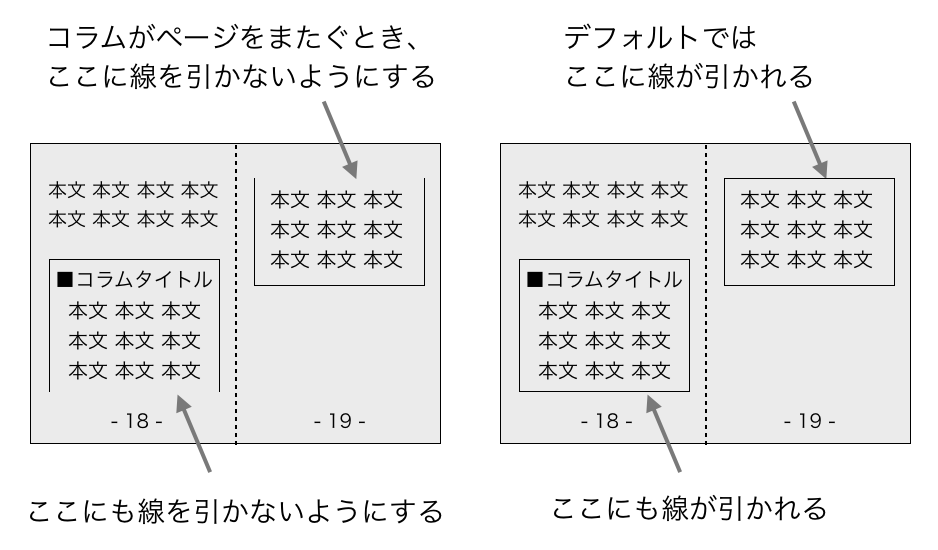
\includegraphics[width=0.8\maxwidth]{./images/chap01-starter/column_openframe.png}%
\reviewimagecaption{コラムがページをまたぐときに横線を入れない}
\label{image:chap01-starter:column_openframe}
\end{reviewimage}

\section{\LaTeX{}のコマンドやスタイルファイルに関する機能}
\label{sec:1-3}
\label{sec-sty}

\subsection*{スタイルシートを追加}
\addcontentsline{toc}{subsection}{スタイルシートを追加}
\label{sec:1-3-1}

Starterでは、次のような独自のスタイルファイルを追加しています。

\begin{description}
\item[sty/starter.sty] \mbox{} \\
Starterのサイトで選択したオプションに従って生成されたスタイルファイルです(Starterのバージョンが上がるたび、このファイルもよく変更されます)。デザインを調整したい場合などはこのファイルを編集するか、後述の\reviewem{sty/mystyle.sty}で上書きしてください。
\item[sty/mytextsize.sty] \mbox{} \\
本文の幅やページ左右の余白を設定するためのスタイルファイルです。PDFのサイズ(B5やA5)を変更する場合は、\reviewem{config.yml}の「\texttt{texdocumentclass:}」を変更してください。
\item[sty/mystyle.sty] \mbox{} \\
ユーザ独自の\LaTeX{}マクロ(コマンドや環境)を追加したり、既存のマクロを上書きするためのファイルです。中身は空なので、自由に追加や上書きしてください。
\item[sty/mytitlepage.sty] \mbox{} \\
タイトルページ(大扉)の内容を表すスタイルファイルです。デザインが気に入らない場合は編集してください。
\item[sty/mycolophon.sty] \mbox{} \\
最終ページの「奥付」を表すスタイルファイルです。デザインが気に入らない場合は編集してください。
\end{description}

\reviewem{sty/mytextsize.sty}と\reviewem{sty/starter.sty}は、どちらも自動生成されます。
なので同じファイルにできそうですが、読み込むタイミングが異なるため、別ファイルにしています。

\begin{starteritemize}
\item \reviewem{sty/mytextsize.sty}は本文の幅や高さを指定するので、他のスタイルファイルより先に読み込まれます。
\item \reviewem{sty/starter.sty}は既存の\LaTeX{}マクロ(コマンドや環境)を上書きするので、他のスタイルファイルより後に読み込まれます。
\end{starteritemize}

\subsection*{印刷用PDFと電子用PDFを切り替える}
\addcontentsline{toc}{subsection}{印刷用PDFと電子用PDFを切り替える}
\label{sec:1-3-2}
\label{bn2iw}

Starterには、印刷用PDFと電子用PDFを切り替えて出力する機能があります\footnote{ただしタブレット用にプロジェクトを作成した場合は、切り替えは無意味です。}。

\begin{description}
\item[印刷用PDF] \mbox{} \\
紙に印刷するためのPDFです。色はモノクロで、またA5の場合はページ左右の余白幅を変更します。
\item[電子用PDF] \mbox{} \\
ダウンロードで配布するためのPDFです。色はカラーで、ページ左右の余白は同じ幅です。
\end{description}

\begin{starternote}{ページ左右の余白幅を変える理由}
\begin{starternoteinner}

印刷用PDFにおいてページ左右の余白幅を変更するのは、本の読みやすさを保ったまま1行あたりの文字数を増やすためです。B5の場合はたいてい十分な紙幅があるので、ページ左右の余白幅は同じままで大丈夫です。A5の場合は見開きで内側の余白幅を確保したまま、外側の余白幅を狭めることで、1行あたりの文字数を増やします。
詳しくは「1.2 レイアウトやデザインに関する変更や拡張」内の\reviewsecref{「奇数ページと偶数ページで左右の余白を変える」}{sec:1-2-5}を参照してください。

当然ですが、このような変更は電子用PDFでは必要ありません。

\end{starternoteinner}
\end{starternote}

設定ファイル\texttt{config{-}starter.yml}の中にある「\texttt{starter: target: }\textit{xxx}」の値が「\texttt{pbook}\footnote{「pbook」はprinting bookの略です。}」だと印刷用PDFが、「\texttt{ebook}\footnote{「ebook」はelectric bookの略です。}」だと電子用PDFが生成されます。初期設定では「\texttt{pbook}」になっているので、デフォルトでは印刷用PDFが生成されます。

またこの値は環境変数\footnote{環境変数とは、コマンドプロセスが参照する外部変数です。環境変数を設定することでコマンドの挙動を一部変更できます。詳しくは「環境変数」でぐぐってください。}\texttt{\textdollar{}STARTER\textunderscore{}TARGET}で上書きできます。具体的には次のようにすると印刷用と電子用のPDFを切り替えられます。

\startercodeblockcaption{印刷用PDFと電子用PDFを切り替える}
\label{}
\begin{starterterminal}\seqsplit{\#\#\# 印刷用PDFを生成(デフォルト)
\textdollar{} rake pdf    \# または STARTER\textunderscore{}TARGET=pbook rake pdf

\#\#\# 電子用PDFを生成(環境変数を使って設定を上書き)
\textdollar{} STARTER\textunderscore{}TARGET=ebook rake pdf}\end{starterterminal}

ただしこの機能では、\LaTeX{}のスタイルファイル(\texttt{sty/starter.sty}や\texttt{sty/mytextsize.sty})の中で行える範囲でしか変更はできません。それ以上のことがしたい場合は、「2.7 その他」内の\reviewsecref{「印刷用と電子用で設定を少し変えるにはどうするの?」}{sec:2-7-2}を参照してください。

\subsection*{ドラフトモードにして画像読み込みを省略する}
\addcontentsline{toc}{subsection}{ドラフトモードにして画像読み込みを省略する}
\label{sec:1-3-3}
\label{8v2z5}

Starterでは画像の読み込みを省略する「ドラフトモード」を用意しました。
ドラフトモードにすると、画像のかわりに枠線が表示されます。
こうすると、(\LaTeX{}のコンパイル時間は変わりませんが)DVIファイルからPDFを生成する時間が短縮されます。

この機能は、図やスクリーンショットが多い場合や、印刷用に高解像度の画像を使っている場合は、特に効果が高いです。

ドラフトモードにするには、\reviewem{config{-}starter.yml}で「\texttt{draft: true}」を設定するか、または環境変数「\reviewem{\textdollar{}STARTER\textunderscore{}DRAFT}」に何らかの値を入れてください。

\startercodeblockcaption{ドラフトモードにしてPDFを生成する}
\label{}
\begin{starterterminal}\seqsplit{\textdollar{} export STARTER\textunderscore{}DRAFT=1  \# ドラフトモードをonにする
\textdollar{} rake pdf

\textdollar{} unset STARTER\textunderscore{}DRAFT     \# ドラフトモードをoffにする}\end{starterterminal}

また「ドラフトモードにしてPDF生成時間を短縮したい、でもこの画像は表示して確認したい」という場合は、「\texttt{//image[][][draft=off]}」のように第3引数に\texttt{draft=off}を指定すると、その画像はドラフトモードが解除されてPDFに表示されます。

\subsection*{コンパイル時の出力を抑制}
\addcontentsline{toc}{subsection}{コンパイル時の出力を抑制}
\label{sec:1-3-4}

\LaTeX{}でコンパイルすると(つまり\reviewem{uplatex}コマンドを実行すると)、通常ではたくさんのメッセージが出力されます。
これはとても煩わしいので、Starterでは出力を抑制するために\reviewem{uplatex}コマンドに「\texttt{{-}interaction=batchmode}」オプションをつけています。

しかしこのオプションをつけると、今度はエラーメッセージが表示されないという問題があります。
つまり、こういうことです:

\begin{starteritemize}
\item 出力を抑制したいなら、\LaTeX{}コマンドに「\texttt{{-}interaction=batchmode}」オプションをつける。
\item しかし「\texttt{{-}interaction=batchmode}」オプションをつけると、エラーメッセージが表示されない。
\end{starteritemize}

なんというクソ仕様でしょう!
このクソ仕様を、Starterでは次のように回避しています。

\begin{starterenumerate}
\item 「\texttt{{-}interaction=batchmode}」オプションをつけてコンパイルする。
\item エラーになったら(つまりコマンドの終了ステータスが0でなければ)、「\texttt{{-}interaction=batchmode}」オプションを\reviewstrong{つけずに}コンパイルし直すことで、エラーメッセージを表示する。
\end{starterenumerate}

今のところ、この方法がいちばん妥当でしょう。

なおこの変更は「\reviewem{rake pdf}」コマンドでのみ行われます\footnote{実装の詳細は\reviewem{lib/tasks/review.rake}を参照してください。}。
「\reviewem{review{-}pdfmaker config.yml}」を実行した場合はもとの挙動(つまりコンパイルメッセージがたくさん出る)になるので注意してください。

ちなみに、\LaTeX{}のコマンドはエラーメッセージを標準エラー出力(stderr)に出してくれません。
クソかよ。

\subsection*{\LaTeX{}コマンドにオプションを追加}
\addcontentsline{toc}{subsection}{\LaTeX{}コマンドにオプションを追加}
\label{sec:1-3-5}

Starterでは、\LaTeX{}コマンド(\reviewem{uplatex})に以下のオプションをつけています。

\begin{description}
\item[\texttt{{-}halt{-}on{-}error}] \mbox{} \\
\LaTeX{}のコンパイルエラー時に、インタラクティブモードにせず、そのままコマンドを終了させるオプションです。
\item[\texttt{{-}file{-}line{-}error}] \mbox{} \\
\LaTeX{}のコンパイルエラー時に、エラー発生箇所の行番号に加えて、ファイル名も出力するようにするオプションです。
\end{description}

指定箇所は\reviewem{config.yml}の「\texttt{texoptions:}」です。

\subsection*{実行する\LaTeX{}コマンドをオプションつきで出力}
\addcontentsline{toc}{subsection}{実行する\LaTeX{}コマンドをオプションつきで出力}
\label{sec:1-3-6}

Starterでは、実行する\LaTeX{}コマンドをオプションつきで出力するように変更しています\footnote{この変更は、\reviewem{lib/tasks/review.rake}で定義されている「\texttt{pdf}」タスクを書き換えることで実現しています。}。
こうすることで、特にエラーが発生した場合にどんなコマンドを実行したかを調べるのに役立ちます。

ただしこれは「\texttt{rake pdf}」を実行したときだけであり、コマンドラインから直接「\texttt{review{-}pdfmaker config.yml}」を実行したときは出力されません\footnote{なぜなら、この変更は「\texttt{pdf}」タスクを書き換えることで実現しているので、\reviewem{review{-}pdfmaker}コマンドには影響しないからです。}ので注意してください。

次が実行例です。
\reviewem{uplatex}コマンドや\reviewem{dvipdfmx}コマンドが、オプションつきで出力されていることが分かります。

\startercodeblockcaption{実行例}
\label{}
\begin{starterterminal}\seqsplit{\textdollar{} rake pdf
compiling chap00{-}preface.tex
compiling chap01{-}starter.tex
compiling chap02{-}review.tex
compiling chap99{-}postscript.tex

[review{-}pdfmaker]\textdollar{} /usr/bin/ruby /tmp/xxx{-}book/lib/hooks/beforetexcompile.rb /tmp/xxx{-}book/xxx{-}book{-}pdf /tmp/xxx{-}book

[review{-}pdfmaker]\textdollar{} uplatex {-}halt{-}on{-}error {-}file{-}line{-}error {-}interaction=batchmode samplebook.tex
This is e{-}upTeX, Version 3.14159265{-}p3.8.1{-}u1.23{-}180226{-}2.6 (utf8.uptex) (TeX Live 2018) (preloaded format=uplatex)
 restricted \reviewbackslash{}write18 enabled.
entering extended mode

[review{-}pdfmaker]\textdollar{} uplatex {-}halt{-}on{-}error {-}file{-}line{-}error {-}interaction=batchmode samplebook.tex
This is e{-}upTeX, Version 3.14159265{-}p3.8.1{-}u1.23{-}180226{-}2.6 (utf8.uptex) (TeX Live 2018) (preloaded format=uplatex)
 restricted \reviewbackslash{}write18 enabled.
entering extended mode

[review{-}pdfmaker]\textdollar{} uplatex {-}halt{-}on{-}error {-}file{-}line{-}error {-}interaction=batchmode samplebook.tex
This is e{-}upTeX, Version 3.14159265{-}p3.8.1{-}u1.23{-}180226{-}2.6 (utf8.uptex) (TeX Live 2018) (preloaded format=uplatex)
 restricted \reviewbackslash{}write18 enabled.
entering extended mode

[review{-}pdfmaker]\textdollar{} dvipdfmx {-}d 5 {-}z 3 book.dvi
book.dvi {-}\textgreater{} book.pdf
[1][2][3][4][5][6][7][8][9][10][11][12]
386603 bytes written}\end{starterterminal}

なお実行結果を見ると、\LaTeX{}のコンパイル(つまりuplatexコマンドの実行)が3回行われていることが分かります。
これはバグではなく、Re:VIEWの仕様です。
理由は、ページ数に変更があっても対応できるようにするためと思われます。

\subsection*{PDF生成を高速化する}
\addcontentsline{toc}{subsection}{PDF生成を高速化する}
\label{sec:1-3-7}

DVIファイルをPDFファイルに変換する「\reviewem{dvipdfmx}」コマンドのオプションを、圧縮率を少し下げるかわりに短時間で終わるようにするよう、設定しました。

具体的には、\reviewem{config.yml}の「\texttt{dvioptions:}」という項目を、Re:VIEWのデフォルトの「\texttt{"{-}d 5 {-}z 9"}」から「\texttt{"{-}d 5 {-}z 3"}」に変更しています。
「\texttt{{-}z 9}」は圧縮率を最大にするので時間がかかり、「\texttt{{-}z 3}」は圧縮率を下げるかわりに短時間で済みます。

PDFファイルのサイズを少しでも減らしたい場合は、「\texttt{{-}z 9}」にしてみてください。

\subsection*{PDFにノンブルをつける}
\addcontentsline{toc}{subsection}{PDFにノンブルをつける}
\label{sec:1-3-8}

印刷所によっては、PDFにノンブルをつけるのが必須です。
たとえば日光企画\footnote{技術書典でいちばん多くのサークルがお世話になっている印刷所。電話対応のお姉さんがとても親切。入稿ページの使い方が分かりにくいので、ほとんどの初心者はお姉さんのお世話になるはず。}さんは、ノンブルをつけないと入稿ができません\footnote{\url{http://www.nikko-pc.com/q&a/yokuaru-shitsumon.html\#3-1}より引用:『ノンブルは全ページに必要です。ノンブルが無いものは製本時にページ順に並び替えることが非常に困難な為、落丁・乱丁の原因となります。』}。

\begin{starternote}{■ノンブルとは}
\begin{starternoteinner}

ノンブルとは、すべてのページにつけられた通し番号です。
ページ番号と似ていますが、ページ番号が読者のための番号なのに対し、ノンブルは印刷所の人が間違えずに作業するための番号です。
具体的には次のような違いがあります。

\begin{starteritemize}
\item ページ番号は読者のためにつけるので、読者から見えやすい場所につける。
   ノンブルは印刷所の人が見えればいいので、読者には見えにくい場所につける。
\item ページ番号は、まえがきや目次では「i, ii, iii, ...」、本文では「1, 2, 3, ...」と増える。
   ノンブルは最初から「1, 2, 3, ...」と増える。
\item ページ番号は、タイトルページや空白ページではつかないことがある。
   ノンブルは、すべてのページに必ずつける必要がある。
\end{starteritemize}

詳しくは「ノンブル」でGoogle検索してください。

\end{starternoteinner}
\end{starternote}

Starterでは、PDFにノンブルをつけるためのrakeタスク「\reviewem{pdf:nombre}」\footnote{\reviewem{lib/tasks/starter.rake}で定義されています。}を用意しています。

\begin{starterterminal}\seqsplit{\textdollar{} gem install combine\textunderscore{}pdf    \# 事前作業(最初の1回だけ)
\textdollar{} rake pdf:nombre}\end{starterterminal}

これで、PDFファイルにノンブルがつきます。

もし\reviewem{pdf:nombre}タスクがうまく動作しない場合は、かわりに\url{https://kauplan.org/pdfoperation/}を使ってください。

\subsection*{rakeコマンドのデフォルトタスクを指定する}
\addcontentsline{toc}{subsection}{rakeコマンドのデフォルトタスクを指定する}
\label{sec:1-3-9}

Re:VIEWでは、rakeのデフォルトタスクが「\reviewem{epub}」になっています。
つまり引数なしでrakeコマンドを実行すると、epubを生成するタスクが実行されます。

これはあまり便利とはいえないし、なによりRubyとrakeをよく知らない人にとっては優しくない仕様です。

そこでStarterでは、rakeの使い方を表示する「\reviewem{help}」タスクを用意し、これをデフォルトタスクにしています。
このおかげで、引数なしでrakeコマンドを実行するとrakeの使い方が表示されます。
このほうが、Rubyとrakeをよく知らない人にとって優しいでしょう。

\startercodeblockcaption{引数なしでrakeコマンドを実行すると、rakeの使い方が表示される}
\label{}
\begin{starterterminal}\textdollar{} rake
rake {-}T
rake all            \# generate PDF and EPUB file
rake clean          \# Remove any temporary products
rake clobber        \# Remove any generated files
rake epub           \# generate EPUB file
rake help           \# + list tasks
rake html           \# build html (Usage: rake build re=target.re)
rake html\textunderscore{}all       \# build all html
rake images         \# + convert images (high resolution {-}\textgreater{} low resolution)
rake images:toggle  \# + toggle image directories ('images\textunderscore{}\{lowres,highres\}')
rake pdf            \# generate PDF file
rake pdf:nombre     \# + add nombre (rake pdf:nombre [file=*.pdf] [out=*.pdf])
rake preproc        \# preproc all
rake web            \# generate stagic HTML file for web\end{starterterminal}

上の表示結果のうち、コマンドの説明文の先頭に「\texttt{+}」がついているのが、Starterで独自に用意したタスクです。

また環境変数「\reviewem{\textdollar{}RAKE\textunderscore{}DEFAULT}」を設定すると、それがデフォルトタスクになります。
たとえば「\reviewem{pdf}」タスクをデフォルトにしたい場合は、次のようにします。

\startercodeblockcaption{pdfタスクをデフォルトタスクにする}
\label{}
\begin{starterterminal}\seqsplit{\textdollar{} export RAKE\textunderscore{}DEFAULT=pdf    \# デフォルトタスクを変更する。
\textdollar{} rake                       \# 引数がないのにpdfタスクが実行される。
compiling chap00{-}preface.tex
compiling chap01{-}starter.tex
compiling chap02{-}review.tex
compiling chap99{-}postscript.tex

[review{-}pdfmaker]\textdollar{} uplatex {-}halt{-}on{-}error {-}file{-}line{-}error {-}interaction=batchmode samplebook.tex
....(以下省略)....}\end{starterterminal}
